%%%%%%%%%%%%%%%%%%%%%%%%%%%%%%%%%%%%%%%%%%%%%
% Template for Master and Bachelor theses   %
% at DSV, an adaptation made by Beatrice    %
% �kerblom of the                           %
%%%%%%%%%%%%%%%%%%%%%%%%%%%%%%%%%%%%%%%%%%%%%
% Template for Doctoral Theses at Stockholm %
% University. The template is based on      %
% the layout an typography used in for      %
% dissertations in the Acta Univeristatis   %
% Upsaliensis series                        %
% Ver 3.0 SU - 2006-09-28                   %
%                                           %
% Erik Siira                                %
% erik.siira@ub.uu.se                       %
% Tel. 471 39 70                            %
%                                           %
% Special thanks to                         %
% Anders K�llstr�m,                         %
% Robert Nyqvist                            %
% and other studens who have used the       %
% former version of this template and       %
% submitted valuable feedback.              %
%%%%%%%%%%%%%%%%%%%%%%%%%%%%%%%%%%%%%%%%%%%%%


\documentclass[12pt,
               a4,
%               swedish,     % Uncomment this line if you write in Swedish
               twoside,
               openright]{book} % Default font 11pt, all pages are
                                % printed the same, new chapter always
                                % begins on a right-hand page.

% \usepackage[frame,a4,center]{crop} % Mount on A4 paper for preview
%% Use this (by uncommenting) if your printer complains that the paper
%% size is not A4.  Don't use it when the final version is produced.


% Package import
% Language, diacritics and hyphanation
               \usepackage[swedish,english]{babel} % Use English
                                                   % and Swedish
                                                   % languages. English
                                                   % default. English
                                                   % hyphenation.
               \usepackage[latin1]{inputenc} % Unix users should
                                             % include this
                                             % package instead of
                                             % ansinew or applemac
                                             % for correct
                                             % handling of
                                             % diacritics.
              % \usepackage[applemac]{inputenc} % Macintosh users
                                                % should include this package 
                                                %instead of ansinew or latin1 
                                                %for correct handling of diacritics.
              % \usepackage[ansinew]{inputenc}  % Windows users include this package 
                                                %instead of applemac or latin1 for 
                                                %correct handling of diacritics. 
\usepackage[T1]{fontenc}
\usepackage{setspace}
\onehalfspace

% Page elements
\usepackage{mathptmx} % Default font for dissertations is Times.
%\usepackage{fourier} % If mathematics don't display well using
                      % Times, then use Fourier.
\usepackage{helvet}  

\usepackage{ThesisSU} % This package is specific for theses
                      % written at Stockholm University. 
                      % Modifications to the classfile and the 
                      % document can be found here.
\ifpdf
   \usepackage[pdftex]{graphicx}
  \else
    \usepackage[dvips]{graphicx}
\fi % Used for figures

\captionsetup{justification=centering} % Centering caption under figures
\usepackage{float}

\usepackage{tabularx}

\setcounter{tocdepth}{5}

\usepackage[colorlinks=true, urlcolor=black, pagecolor=black,
linkcolor=black, citecolor=black, filecolor=black,
menucolor=black, pdfpagelayout=TwoColumnRight, pdfstartview=FitH,
plainpages=false,
pdfpagelabels]{hyperref} % Use this package to obtain links in the
                         % electronic version of the document. All
                         % hyperlinks and other links
                         % should be black. Page view is set to
                         % Fit Width and page layout is set to
                         % display the document spread.  Make page
                         % anchors using the formatted form of the
                         % page number.  Set PDF page labels;
                         % i.e., write the value of \thepage to
                         % the PDF file so that Acrobat Reader can
                         % display the page number as (say) 'ii (4
                         % of 40)' rather than simply '4 of 40'.

% Bibliographic information
% Filling in this bibliographic information facilitates the
% processing of this document.

% Insert linebreaks if necessary

% Just leave the posistion blank for any information that doesn't
% apply for your thesis, e.g. if your thesis doesn't have a subtitle:
%
% \newcommand{\thesisSubtitle}{}




% Abstract and titelpage

\firstAuthorFirstName{Leon}                % First author given name
\firstAuthorSurname{Hennings}                 % First author surname
\secondAuthorFirstName{Kamyar}              % Second author given name
\secondAuthorSurname{Sajjadi}                % Second author given name

\firstAuthorEmail{leon.hennings@gmail.com}              % First author's e-mail address
\secondAuthorEmail{kasa5879@student.su.se}             % Second author's e-mail address

\thesisTitle{Re-engineering the MediaSense Platform towards Resource Constrained Devices}                   % The title of the thesis
\thesisSubtitle{RPC-based Daemon Approach} % The subtitle of the thesis 

\thesisSubject{Computer and Systems Sciences}   % May be changed
                                                % to e.g. Human-Computer 
                                                % Interaction or other 
                                                % suitable for your thesis 
\thesisIsKind{Bachelor}                           % Change to Bachelor if suitable
\theYear{2013}
\thesisCred{15}                                 % Change to 15 if Bachelor
\thesisAdvisor{Jamie Walters}
\thesisAssistantAdvisor{}                       % Name of Assistant Advisor,
                                                % if you have one
\thesisExternalAdvisor{}                        % Name of External Advisor,
                                                % if you have one

\thesisReviewer{Iskra Popova}
\semester{Spring}
\swedishTitle{}

                                               % The abstract text comes
                                               % here. Not more than 300
                                               % words. No empty lines.                                     
\abstracttext{Computers are becoming pervasive in our society through the use of tablets, smartphones, computers embedded in home appliances and media devices. These devices are becoming more connected, creating an Internet of Things. The Internet of Things will make use of all collected data currently stored separately in devices and allow for a new type of immersive applications by utilizing users' data from several sources. 
MediaSense as an Internet of Things middleware allows for communication between devices and distributed sharing of context information. MediaSense in its current form it is not 
geared towards smaller, portable computers that are making up the Internet of Things. This project applies a design science methodology for re-engineering the platform to make it usable on ubiquitous devices. This thesis propose a redesign intended to create a shared background service, a so called daemon, of the MediaSense platform so the functionality of sharing and storing sensor data is shared among the applications using it. To implement this behavior, a type of inter-process communication had to be chosen to allow the applications to communicate with the platform. The Java implementation of Remote Procedure Call called Remote Method Invocation was chosen. The new version of MediaSense was designed and developed according to the requirements outlined by the lead developer of MediaSense. The redesign resulted in lower memory usage and less CPU time when running more than one application. 
This discovery will make Internet of Things middleware possible to use on ubiquitous devices and enable several immersive applications to run simultaneously on one device.}



\keywords{Immersive Participation, Context Awareness, Pervasive Computing, Ubiquitous Computing, Internet Of Things, Middleware, MediaSense, Distributed, Inter-Process Communication, Remote Method Invocation}


 % This file should be edited by the author.


\begin{document}
  
    \frontmatterDSV % Sets the frontmatter (Title page(s), abstract, keywords, etc.)
    
    \tableofcontents
    
    % Optional tables
    \listoftables
    \listoffigures

    % This includes the "Instruction" and "Problem and Solutions"
    % files. After reading it, remove it from Thesis.tex.
    \chapter{Introduction}

    \chapter{Background and Theory}
This chapter explores the two general areas of Computer Science that are considered when developing and deploying an Internet of Things platform supporting resource constrained devices. Firstly, we describe the general area of Immersive Participation and its constituent theories around pervasive computing. Secondly we look at the deployment of pervasive middleware in the distributed computing paradigm more closely examining the MediaSense platform as a concrete realisation of this approach. Additionally, we discuss the general trend of pervasive and ubiquitous computing towards resource constraint devices. Finally, we look at the inter procedure communication and more specifically remote method invocation as the theory for extending the MediaSense platform in order to solve the problem shown in section \ref{problem}. 

\section{Immersive Participation}
Immersive participation is focused on participation on the Internet via ubiquitous computing and context-awareness. It enables people, places and things to connect to each other to create Immersive Participation Environments. Immersive Participation Environments provides users with context-awareness everywhere which makes the users participate as if they are in a virtual world with places, things and people in it. Common examples of Immersive Participation Environments today include Google Ingress \cite{ingress} where users join teams and compete with other teams in a virtual world where they need to take over real world artefacts, TURF \cite{turf} where users capture real world places and gain points and RATS Theatre's \cite{rats} application called Maryam \cite{maryam} which is an interactive theater where audio clips is triggered depending on the user's Global Positioning System (GPS) location.

Larger scale immersive applications will benefit from scalable distributed information sharing and also remove bottlenecks and dependencies on centralized web portals on the internet.
The way humans interact with each other and things around them will change when sensor information can be shared and accessed ubiquitously. Creating immersive environments that blend the natural world with a seamless internet of things require that we are able to understand the situation of the users in real-time this understanding is termed context awareness.

\section{Context Awareness}
Improving the computers ability to access and understand a user's circumstances give developers more information for creating  applications that respond and adapt to the user. A way to accomplish this is to not only use data given by the user, but also use context information from the user's environment. According to Dey in \cite{dey2001understanding}, the definition of context is:

\begin{quotation}
\centering
Context is a combination of any information that can be sensed or received by an entity which is useful to catch events and situations.
\end{quotation}

In other words, context is information from an entity that gives specific information to increase the understanding of an events environment. An entity can be a person, place or an object that is relevant for the interaction. 

One way of generating and sharing this context information on a large scale is through the use of smart telephones and other ubiquitous computing devices. One such smartphone is the a Google Nexus 4 \cite{GoogleNexus} which contains, among other things, an accelerometer to detect acceleration, a GPS to receive location data, a gyroscope to detect rotation, a barometer to detect air pressure and a compass for direction and navigation. By applying sensor fusion \cite{Elmenreich02sensorfusion} other context data can be attained. The phone will collect context-information from its GPS sensor and based on this location be able to give directions. With this extra context information, we can create applications that are context aware. This idea of context awareness is summarized by Dey in \cite{dey2001understanding} as: 

\begin{quotation}
\centering
A system is context-aware if it uses context to provide relevant information and \slash or services to the user, where relevancy depends on the user's task.
\end{quotation}

An example of context-awareness in applications is Google Latitude \cite{GoogleLatitude}, where it's possible to see your friends' location on a map, as shown in figure \ref{googlelat}. Other good examples include applications on smartphones and tablets which rotate the image on screen based on the device's physical orientation as shown in figure \ref{androidorientation}.

\begin{figure}[t] % To force on specific place use H
	\centering
    	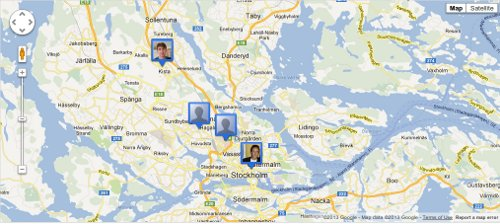
\includegraphics[scale=0.75]{part_2/context_awareness/latitude_pic.jpg}
		\caption{A picture of Google Latitude showing contacts shared positions.} 
		\label{googlelat}
\end{figure}

Context awareness can change classical scenarios into intelligent responsive scenarios by using context information to determine a behavior, such as turning on lights in the house when the user approaches home. Context awareness on a massive scale is gradually enabled by the advances in pervasive and ubiquitous computing.

\begin{figure}[t] % To force on specific place use H
	\centering
    	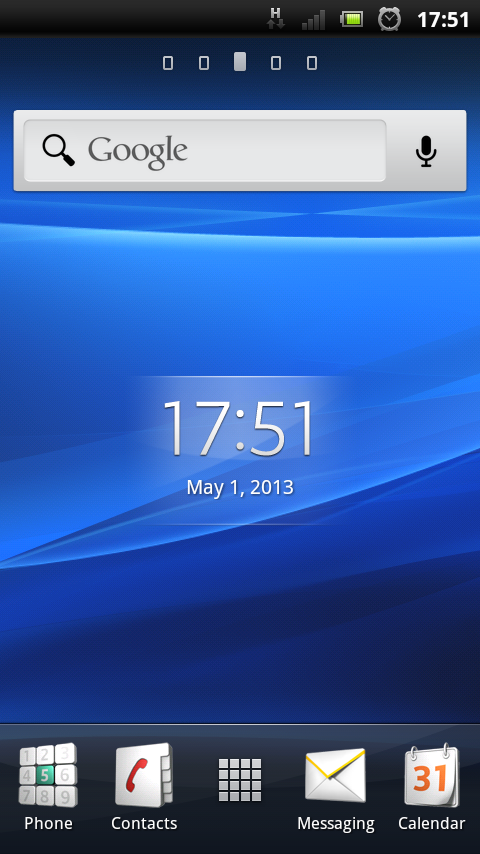
\includegraphics[scale=0.20]{part_2/context_awareness/screenshot_2013-05-01_1751.png}
    	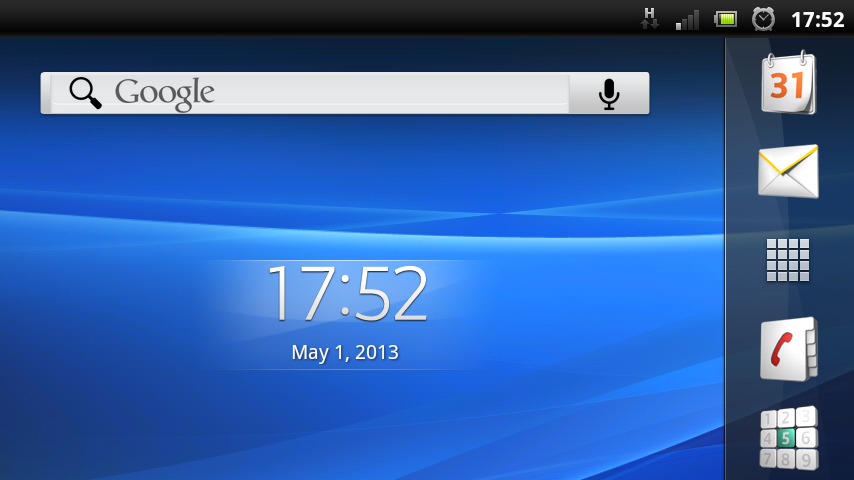
\includegraphics[scale=0.20]{part_2/context_awareness/screenshot_2013-05-01_1752.png}
		\caption{Android homescreen on a Sony Ericsson Xperia PLAY rotates based on context information from its sensors when the phone is 	physically rotated.} 
		\label{androidorientation}
\end{figure}

\section{Pervasive \& Ubiquitous Computing}
Pervasive and Ubiquitous computing describes the philosophy of "everything everywhere computing". To build context-aware applications context information is needed and ubiquitous computing can be used to make collection of this data possible.
Computers today are everywhere; in phones, TVs, cars, kitchen machines, watches, etc. Jens Malmodin et al. \cite{fehske2011global} predicts that 50 billion devices will be connected together by 2020. When computers become pervasive and ubiquitous it becomes important to make the computers themselves smart and easy to use instead. According to Mark Weiser in \cite{237456} the goal of Ubiquitous is 

\begin{quotation}
\centering
[...] the enhancing computer use by making many computers available throughout the physical environment, but making them effectively invisible to the user.
\end{quotation}

According to The Swedish Data Inspection Board \cite{datainspect}, ubiquitous computing is a new computer era. In the past one human only had one computer, so called personal computer (PC). In the last years this have been changing. Computers have been integrated into artefacts that humans use in their everyday life. Shoes can contain a computer chip that collects data about your running \cite{saponas2006devices}. With ubiquitous computing places and physical objects will be connected and communicate with each other and humans. 

If computers will be everywhere, they must be as small as possible. They also need to be cheap and be low-powered computers \cite{datainspect}. An example is the Raspberry Pi, a credit card sized computer that can be run with 4 x AA batteries. According to Moore's Law, in the coming years devices will be smaller, more powerful and they will be much cheaper \cite{591665}. This gives a good chance that computers which already are embedded in all things around us will be powerful enough to run multiple context aware applications.

%\section{Tendency Towards Resource Constrained Devices}
Alan Messer et al \cite{alanmesser} have identified a problem with the concept of pervasive computing. Peoples vision is to execute a service on any device without worrying about whether the service is designed for the device. Alan Messer et al suggests that it will be difficult to create a service that can be run on all devices due to the resource constraints on different devices. Devices differ from each other with respect to their processing power, available memory or network access, hence services need to be tailored to work on different devices.


A lot of existing computer software was first developed for computers with high resources. When software runs on a computer with low resources it needs a redesign to fit on the device. The operating system Android is built on Linux which was an operating system that first was used on personal computers. Android Inc redesigned the operating system to fit it on smartphones. The same goes for Microsoft that has developed a version of Windows for tablets and smartphones. Applications like Netflix, Google Chrome and Utorrent have been redesigned to fit different devices. Software can sometimes be run on a device for which it wasn't designed to run on, but the software is not tailored for those devices and will therefore be less efficient causing reduced performance.


%\section{Tendency Towards Resource Constrained Devices}
Alan Messer et al \cite{alanmesser} have identified a problem with the concept of pervasive computing. Peoples vision is to execute a service on any device without worrying about whether the service is designed for the device. Alan Messer et al suggests that it will be difficult to create a service that can be run on all devices due to the resource constraints on different devices. Devices processing, memory, network, power capacities differs from each other and services need to be tailored to fit on different devices. 

A lot of existing computer software was first developed for computers with high resources. When software runs on a computer with low resources it needs a redesign to fit on the device. The operating system Android is built on Linux which was an operating system that first was used on personal computers. Android Inc redesigned the operating system to fit it on smartphones. The same goes for Microsoft that has developed a version of Windows for tablets and smartphones. Applications like Netflix, Google Chrome and Utorrent have been redesigned to fit different devices. Software can sometimes be run on a device for which it wasn't designed to run on, but the software is not tailored for those devices and will therefore be less efficient causing reduced performance.

\section{Applications Using Context Information}
To build this big network of context aware applications that interact with users without them knowing it, some conditions must be understood. Because of the mobility of the devices the context information need to be collected and shared through wireless network. Moreover, the infrastructure for an Internet of Things platform have to scale well to increase amounts of users and have to always be available to these users \cite{Kanter539187}.

Another condition to consider is the large number of applications that should be able to run on a single ubiquitous device. The ubiquitous devices have limited performance, even if the evolution of the hardware is going forward. Due to their size it is important for an application to be lightweight. Ubiquitous computer devices have limited processing capability, small memory space and have limited battery time. The capability of processing is limited which make them not well suited for computation of intensive tasks. A ubiquitous device also has limited amount of available memory. This two conditions makes it more important to have lightweight applications and services on ubiquitous devices. As mentioned before battery time is also limited, for example the battery time is decreased whenever the device has network communication. Therefore it is important to make the applications and services efficient in the use of network communication. 
If we run a context-aware application on a Raspberry Pi we need to consider that the device only has 512 MB RAM and that this device should be able to run several instances of similar applications so the footprint from the network communication need to be reduced. 

The applications also need near instant access to context-information. Context-information need to be accessed in real-time to provide updated data from sensors. This cannot be provided with a centralized solution \cite{TheMediaSenseFramework}. Real-time delivery of context-information between endpoints is important to existing and future mobile applications. 

\section{Sharing the Information}
As the network of ubiquitous computers grows bigger, the amount of context information will increase as well, and it becomes necessary to understand how this information can be shared. When billions of users and applications is connected to the infrastructure, it is important to get the most effective and scalable solution for storing and sharing this kind of data. Applications will need to be able to access data in real-time, so the users get the most updated context information. 

To share the information ubiquitous devices need a middleware, a platform that can run on the ubiquitous devices and enable information sharing. This middleware should be able to provide the functionality for collecting and sharing context information, it also needs to be able to share the context information in real-time. Because of the ubiquitous devices resource limitations it needs to be lightweight and use the resources in an efficient way. There are two approaches this middleware could use to share context information, centralized and distributed.

\subsection{Centralized}
With centralized middleware solutions, the data is hosted and managed on a server, and if a device needs to store or access context information it has to connect to this server. One advantage of the centralized approach is that a server can be updated, with new hardware and software, to improve its performance. 
However, a server can only handle a certain amount of requests per second. To handle the larger quantities of requests, more servers will be required causing the costs to increase with the amount of users. A centralized approach is vulnerable to failures like attacks and crashes. When the server goes down, users won't be able to retrieve context information. Some examples of Internet of Things middleware which use this approach are SenseWeb \cite{senseweb} and Xively \cite{xively}.

%\begin{figure}[t]
%	\centering
%    	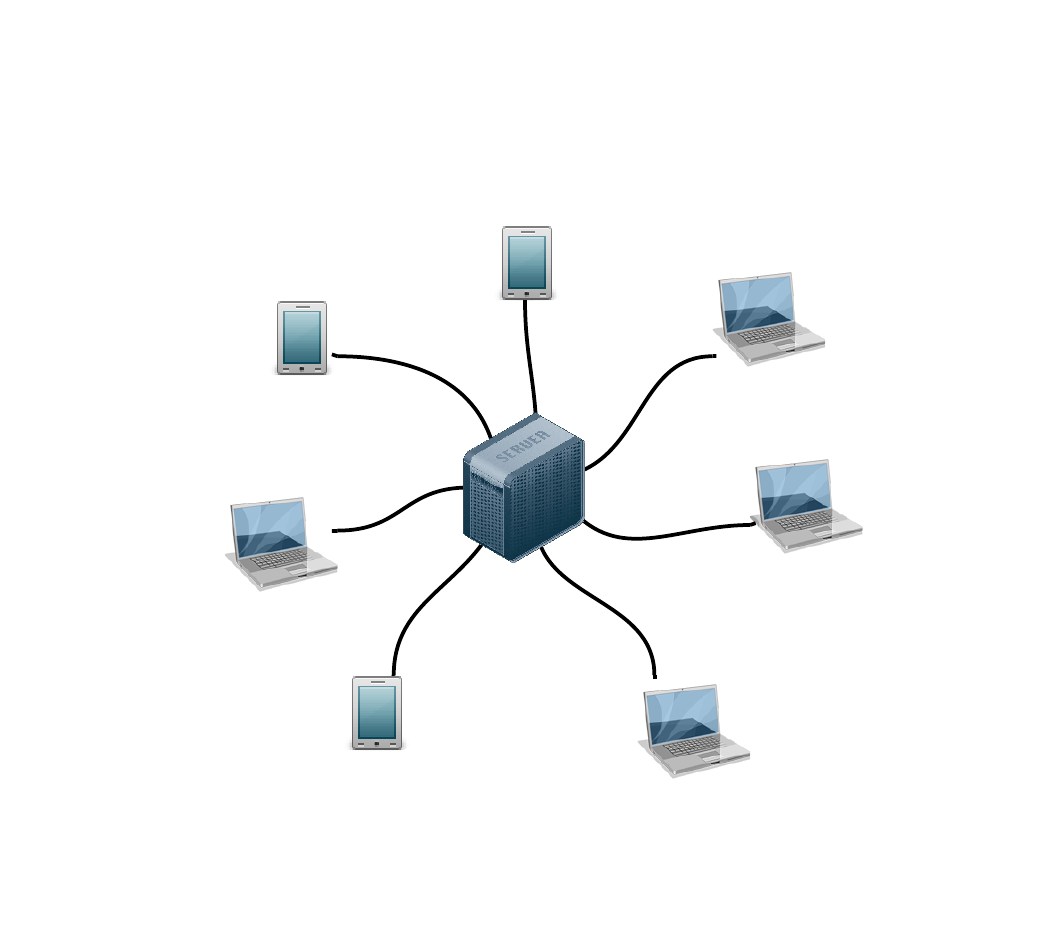
\includegraphics[scale=0.25]{part_2/sharing_the_information/Centralized.png}
%		\caption{Overview of a centralized network} 
%\end{figure}

\subsection{Distributed}
Distributed solutions allow computers / nodes to communicate with each other and share information and resources without using server computers. This is commonly used in file sharing software applications, such as Gnutella. Distributed solutions are more reliable and lack a single point of failure. Distributed solutions scale well compared to centralized solutions. Ubiware \cite{osterle2010memorandum} and MediaSense \cite{TheMediaSenseFramework} are both distributed Internet of Things middleware. 

%\begin{figure}[t]
%	\centering
%    	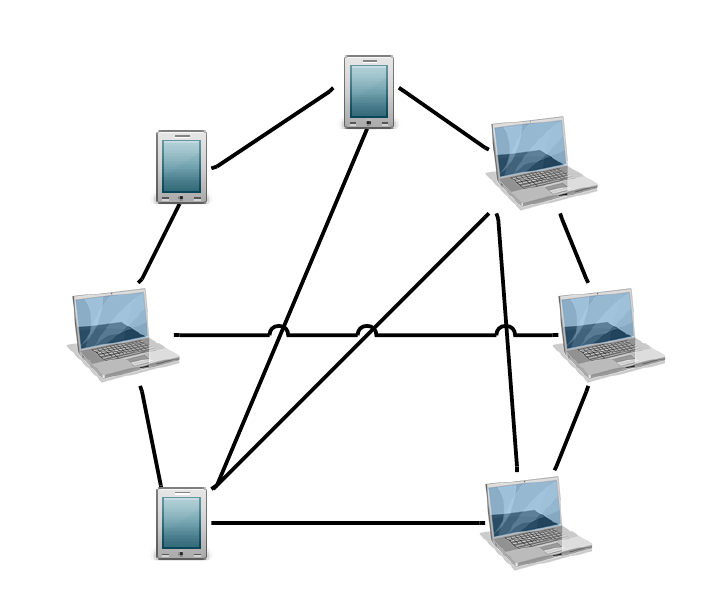
\includegraphics[scale=0.25]{part_2/sharing_the_information/Decentralized.png}
%		\caption{Overview of a decentralized network} 
%\end{figure}

\section{MediaSense}
MediaSense is a distributed middleware platform for the Internet of Things. It provides a scalable platform with a real time access to context information \cite{Kanter539187}. MediaSense allows support for applications and services to collect and share context information. This in turn enables users to focus on developing applications and services without needing to focus on how the context information is shared and how the layers in the platform is interacting with each other \cite{Walters413794}. 

\subsection{Distributed}
MediaSense is using a distributed peer-to-peer overlay to connect all the endpoints in the network. Context information is then persisted and shared in real-time among the nodes in the network. Each node in the network is both a producer and consumer enabling bidirectional access to context information. The overlay used is P-Grid \cite{aberer2003p}. With a lot of users running applications and sharing context information it is critical that the overlay structure is reliable and scalable \cite{aberer2003p}. P-Grid is self organizing allowing it to scale well. 

\subsection{Applications}
MediaSense is written in the programming language Java and provides an API that can be used to communicate with the platform. The communication from one platform on a device to another device running the platform is done with messages. The API provides methods for registering new context information and find nodes holding specific context information. Each node attached to the network generates information on a continual basis that is accessed and used by other nodes wishing to do so. In order to do this each node register UCIs (Universal Context Identifier). The UCI is stored in the distributed network and other nodes can resolve this and get the address where some required information is stored. When a MediaSense instance gets a message the dissemination layer in MediaSense handles this message and sending it to the application. The dissemination layer acts like a router delivering messages to the right place. Applications have a method for handling messages that is routed from the dissemination layer. 

\begin{figure}[t]
	\centering
	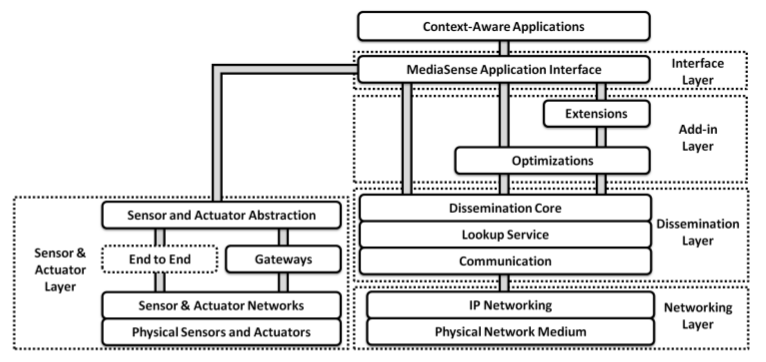
\includegraphics[scale=0.50]{part_2/mediasense/ms_arch.png} 	
	\caption{MediaSense component architecture \cite{Kanter539187} }
\end{figure}

\subsection{Messages}
As mentioned MediaSense communicates with messages. Applications can register what messages they are interested in. When the platform gets a new message from another node in the network the message will be handled by the dissemination core which then sends the message to the application on the platform interested in this message. There are several types of messages. The table \ref{tab:table} shows the primitive messages that are available for registering and retrieving information. 

\begin{center}
\begin{table}
    \begin{tabularx}{\textwidth}{ | l | X |}
    \hline
    Message name 		& 		Description \\ \hline
	REGISTER UCI 		& 		Registers a UCI along with the node which is responsible for it. \\ \hline
	RESOLVE UCI 		& 		Resolves a UCI to the node which is responsible for it. \\ \hline
	GET 				& 		Fetches the current context value from the node responsible for a UCI. The reply is sent using a NOTIFY. \\ \hline
	SET 				& 		Changes the current status of an actuator in an end point. \\ \hline
	SUBSCRIBE 			& 		Makes a subscription request to the node responsible for a UCI, The node then sends a NOTIFY message containing the current context value, either at regular intervals or when the value changes. \\ \hline
	NOTIFY 				& 		Notifies an interested node of the current context value associated with a specified UCI. \\ \hline
	TRANSFER 			& 		Requests the manager of a resource to transfer responsibility to another node. This might be full responsibility or partial, where the requester re-creates a copy of the resource permitting improved real time performance. \\ \hline
    \end{tabularx}
	\caption{Primitive messages in MediaSense}
	\label{tab:table}
\end{table}
\end{center}


\subsection{MediaSense Execution}
When an application wishes to use the MediaSense platform, the application must initialize and use its own instance of MediaSense. Therefore a user running two application at the same time must initialize two instances of the platform. Every instance of MediaSense is seen as a separate node, so if we have two instances of the platform on one device this device is acting as two nodes in the network. This is misleading because one node in the network should be one device and not one application.

\begin{figure}[t]
	\centering
    	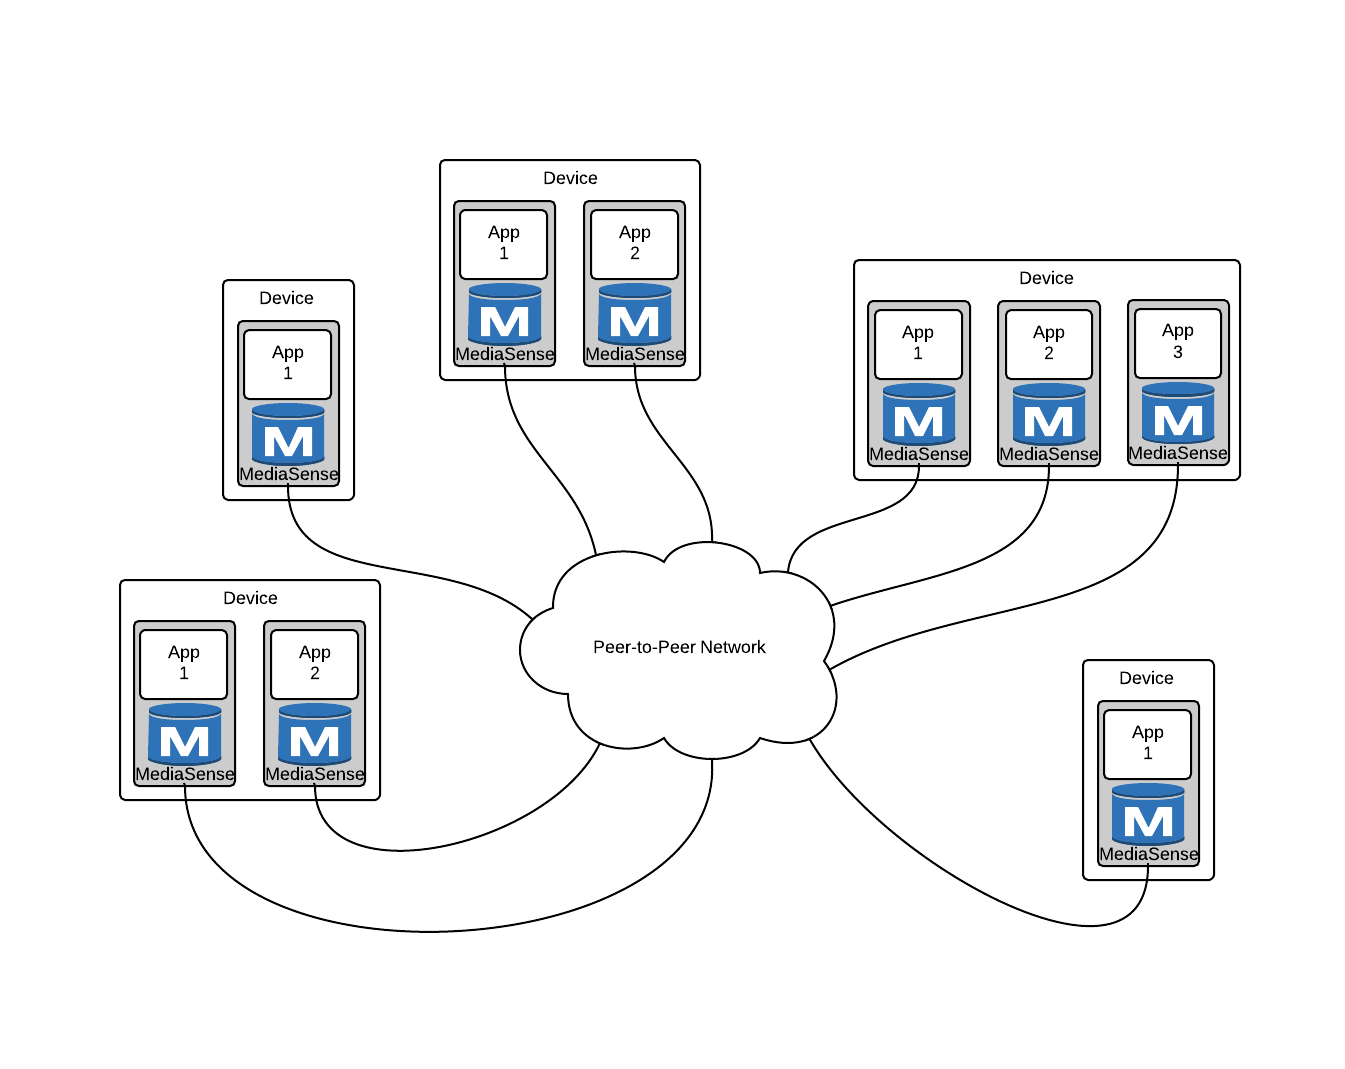
\includegraphics[scale=0.25]{part_2/mediasense/several_nodes_on_one_device.png}
		\caption{Figure showing how the instances of MediaSense is connected to the network} 
\end{figure}

Each instance of MediaSense requires that a new port be opened so the network layer can communicate with other nodes in the network. This means that if the user is behind a NAT or a firewall the user needs to open up new ports for every instance of MediaSense. The amount of open ports is equal to the amount of applications running on a device. This is a security issue. With more ports opened the device that is running the platform is more vulnerable. Not only that the device will be more vulnerable, when a user need several instances of MediaSense and every instance need its own port the network usage will increase. This can affect the battery time of low resource devices in a negative way.

One more thing to consider with an application invoked platform is that the memory usage will increase. Every instance of MediaSense need to use a specific amount of memory. If the platform is running on a resource constrained device this will limit the number of applications running on the device, because of the several instances of MediaSense. This is contradictory to the requirement defined by Kanter et al. \cite{Kanter539187} that Internet of Things Middleware should be lightweight.

To make MediaSense more efficient we need to reduce the resource footprint, without losing  the functionality. This can be done in several ways. One way is to change the overlay architecture and use a centralized approach for sharing and collecting context information. This solution will make every application connecting to a centralized server or to use a internet portal, for example RESTful API to access the data. The problem with this is that they are centralized and therefore not well scalable and we will lose the functionality of P-Grid. They are also dependent on DNS which means that applications expect that the centralized server are always available. As mentioned before centralized solutions are more vulnerable and can be attacked with Denial-of-service attacks. If the centralized server is having DNS errors the context information can not be accessed and shared to other applications and the applications is usable. Examples of Internet of thing services using this architecture is SenseWeb and Sensei. This two examples is using centralized web-services for sharing context information which makes them having the mentioned issues and are therefore not a good solution for an Internet of things service.

\begin{center}
\begin{table}
    \begin{tabularx}{\textwidth}{ |X|X|X|X| }
    \hline
    Number Of Applications 								& Memory Usage 									& CPU Time							& Threads\\ \hline
    1 													& 70.4 MB 										& 2.70 								& 30 \\ \hline
    2 													& 139.2 MB										& 5.34 								& 60 \\ \hline
    3 													& 213.04 MB										& 8.72 								& 90 \\ \hline
    4 													& 286.5 MB										& 12.88 							& 120 \\ \hline
    5													& 360.2 MB										& 15.43  							& 150 \\ \hline
    6													& 430.3 MB										& 18.82  							& 180 \\ \hline	
    7													& 505.3 MB										& 21.54  							& 210 \\ \hline
    8													& 574.1 MB										& 24.85  							& 240 \\ \hline
    9													& 648.3 MB										& 27.84	  							& 270 \\ \hline
    10													& 718.3 MB										& 31.25  							& 300 \\ \hline
    \end{tabularx}
   	\caption{This table shows how much resource is in use when MediaSense is running}
	\label{tab:test_table}
\end{table}
\end{center}
\section{Shared Resources to Reduce Resource Costs}
The resources of computers can be used in an effective way if the applications have resource consuming components located in a shared service. A shared service can act like a container where components like databases, calculations and network communication can be shared between all processes. One example of shared resources are web browsers. In the late 1990s and early 2000s web browsers could only visit one web page and to view multiple web pages simultaneously new windows had to be opened. Tabbed browsing or TDI (tabbed document interface) of web pages was popularized by Mozilla FireFox in 2003 and made it possible to have several web pages opened in one window. Tabbed browsing allows web browsers share services between the tabs displaying web pages. Examples of such services in web browsers are JavaScript engines, rendering engines, plug-ins, extensions, et cetera. 
MySQL has a shared service for all databases running on a server, a so called daemon, which handles access to all databases on the server. For example, the communication with MySQL is handled by the shared service which listens to a TCP port. When the service gets a request to this port it forwards it to the addressed database. If MySQL instead had one service for every database, one network layer is needed for every database which increase the resource usage. 

The tendency to gather resource consuming processed in one place and share access to them between many processes is the basis of the client-server model. Examples of such behaviours are numerous and prominent within the world wide web. Google's massive indexed database of web pages can be queried by millions of users at a time. This forces google to have large and powerful data centers to accommodate the users instead of each user downloading a copy of Google's database and querying it locally. Spotify's large collection of music can be accessed by users and streamed to a client giving access to approximately 80 terabytes (20 million songs at an average size of 4MB) of music for which the storage costs alone would be unfeasible for the average user by todays standards.
\section{Inter-Process Communication}
Inter-process Communication (IPC) is a term describing communication between two processes through a shared interface. There are a number of variations of IPC. In operating systems like Unix and Windows there are a mechanisms for local IPC such as files, sockets, pipes, shared memory and semaphores. 
Inter-process communication using files is simply done by two processes reading and writing to one or more files. Pipes are a way of directing the output of one program to the input of another program. A variation of pipes are named pipes, also called FIFO (first in first out) which are system persistent pipes, often represented as files \cite{Lewandowski97interprocesscommunication}. Sockets are software abstractions to create a bidirectional channel between processes. They come in two variations, datagram sockets and stream sockets. Datagram sockets are faster than stream sockets but less reliable \cite{Lewandowski97interprocesscommunication}. Shared memory allows two processes to access the same memory and semaphores are used to signal availability of a resource between processes to avoid information loss, so called race conditions, while writing to the same block of memory from two different processes.

For communication between applications there are Inter-process communication implementations supporting communication with applications running on remote computers through interfaces of a higher abstraction than those for local IPC. These can also be used locally but the abstractions come at a cost in resources.

Remote IPC can be done in two ways unicast and multicast. Unicast is when the communication is sent from one entity and received by another entity. An example of unicast remote IPC is Remote Procedure Calls, RPC. Multicast is when the communication is sent from one entity and received by a group of entities. An example of multicast IPC is message passing which is used by the MediaSense platform to communicate between nodes over the Internet.

\subsection{Message Passing}
Message passing performs IPC by sending and receiving messages. Received messages are placed in a queue and are handled asynchronously.
The messages contain data which is used to determine the action or response. This allows the receiver to prioritize some messages. Message passing provides few abstractions for the developer and requires the data to be marshalled before sending messages and unmarshalled before receiving messages. 

The Message Passing Interface, MPI \cite{mpi3stand}, is one such standardized message passing implementation. Sending and receiving operations in MPI can be either blocking or non-blocking. Blocking send and receive operations wait for the application buffer to be free for reuse before returning to prevent race conditions, while non-blocking messages allow the process to proceed as soon as possible.

\subsection{Remote Procedure Calls}
Remote Procedure Calls (RPC) are a form of IPC that allow one process to invoke a callable unit \cite{Eac} located in another logical or physical space. Usage of RPC makes it possible to both interact with programs running on the same physical memory and with applications located within the same network. RPC is an abstraction built on top of message passing to enable calls to remote procedures as if they were made locally.
RPCs are unicast and synchronous, the sender waits for a response from the recipient before continuing the execution. Remote procedure calls are handled as if the calls were done locally, the calling process waits for a return value before proceeding, see Fig. \ref{rpc}.

Bruce Jay Nelson first defined Remote Procedure Calls as
\begin{quotation}
\centering
[...] the synchronous language-level transfer of control between programs in disjoint address spaces whose primary communication medium is a narrow channel.  \cite{Nelson:1981:RPC:910306}
\end{quotation}

\begin{figure}[t]
		\centering	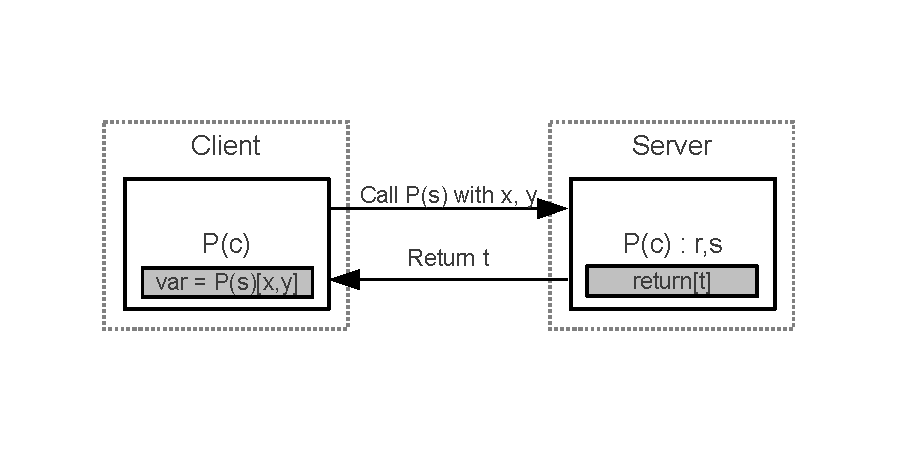
\includegraphics{part_2/remote_procedure_calls/rpc.pdf}
		\caption{Abstract of the events involved in remote procedure calls from a user perspective.
The procedure P(c) in the Client calls procedure P(s) located at the Server. The procedure P(s) receive two arguments r and s and return the value t which is stored in variable var back in the client.}
		\label{rpc} 
\end{figure}

When using remote procedure calls, one process is considered the server and one the client. The client is the caller process and the server receive and handle the process and then returns the value. The client and server both have stubs, server-side stubs are called skeletons. Stubs are modules in charge of marshalling the calls, which means packing the parameters of the call in a way that allows them to be stored or transferred via TCP or UDP \cite{rfc5531}. 
The events that occur when a client invokes a remote procedure call start with a call to the client's stub are shown in \ref{rpcflow}. The client stub receive the parameters from the local call and then marshalls. The marshalled data is then sent to the server by the the client's operating system. The server operating system receives the message and sends it to the skeleton. The skeleton unmarshalls the message  to obtain the parameters and invokes the local version of the procedure with the parameters. The server's procedure returns a value which is then sent to the skeleton. The skeleton then in turn marshalls the return value and sends the marshalled data back to the client. The client receives the message, the client stub unmarshalls the return value which then is sent back to the client's procedure \cite{Lewandowski97interprocesscommunication}. RPC implementations often is language specific. Some implementations, like XML-RPC and 
JSON-RPC use a common format for describing objects and can therefore be used cross-platform.

\begin{figure}[H]
		\centering	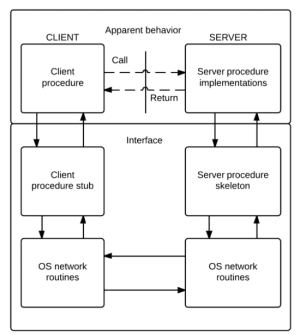
\includegraphics{part_2/remote_procedure_calls/Rpcflow300.png}
		\caption{The flow of a RPC}
		\label{rpcflow} 
\end{figure}

\subsection{Remote Method Invocation}
Remote method invocation (RMI) is a Java implementation of RPC with support for Java objects and allows entire objects to be passed and returned as parameters instead of only primitive data types. These objects can be dynamically loaded in the receiving Java Virtual Machine and can therefore be of an object type unknown to the receiver. RMI requires objects to be RemoteObjects, a remote object must implement a remote interface to support remote invocations. When a remote object is sent to another Java Virtual Machine it is sent as a remote stub to the receiving remote.
RMI relies on a registry to find other remote objects which have to be registered with a name. Other objects can then do a lookup on the registered name to get a reference to the Remote object. RMI registries can be shared between multiple JVMs on the same machine which facilitates communication from newly created processes to persistent ones.

\begin{figure}[H]
	\centering
    	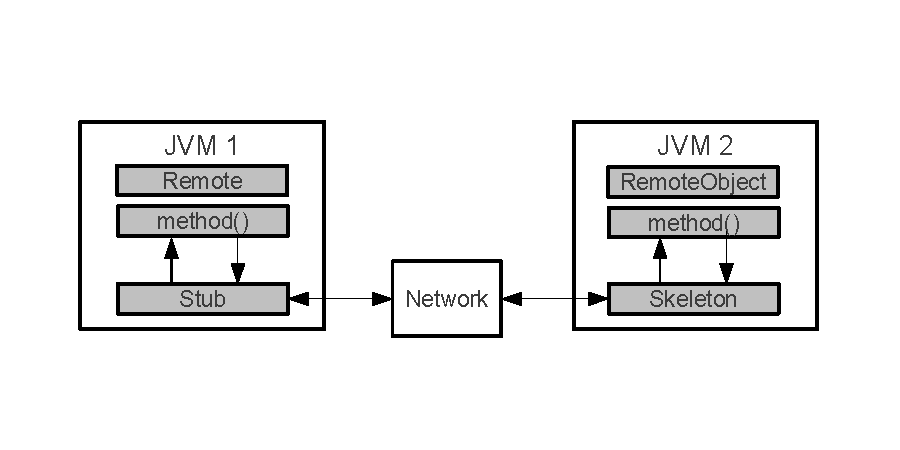
\includegraphics{part_2/remote_procedure_calls/rmi.pdf}
		\caption{The sequence of events in a method invocation with RMI.}
		\label{rmi} 
\end{figure}

\subsection{CORBA}
Common Object Request Broker Architecture is an object-oriented Remote Procedure Call mechanism. Corba is implemented in many different programming languages. This enables softwares written in different languages to communicate with each other. This is done with a language neutral API. CORBA uses an Object Request Broker which provides the mechanism required for distributed objects to communicate with each other. The Object Request Broker determines the location of target object, sends a request to that object and then returns a response back to the calling object. This communication is done over TCP/IP. However, in CORBA it is not possible to bind an Object Request Broker to a specific port. If the client is behind a firewall there is no option to change the port and use another port. This makes Corba firewall unfriendly.


    \chapter{Method}
To be able to solve the problem it is necessary to rethink and redesign core-components of the an existing middleware. Using traditional quantitative or qualitative research methods would not involve any actual designing. These research methods produce data based on past or present conditions and don't allow researchers to develop artefacts.
Design science research differs in one major way from qualitative or quantitative empirical studies. Where empirical studies focus on finding patterns in the past or present of an industry or a field, design science is intended to design and develop new solutions to actual problems \cite{bider2012design} and aims to improve and create artefacts that can improve the world \cite{johannesson2012design}. 
Design science is well suited for this problem because it involves a step where requirements are identified and a design and develop action where the researchers develop an artefact based on the requirements. Lastly there is an evaluation action where the artefact is evaluated based on the requirements to see if they have been met and thus if the artefact solved the problem. Consequently design science is a good method to use for this problem where a redesign of an existing middleware for the Internet of Things is needed.

\begin{figure}[h!]
	\centering
    	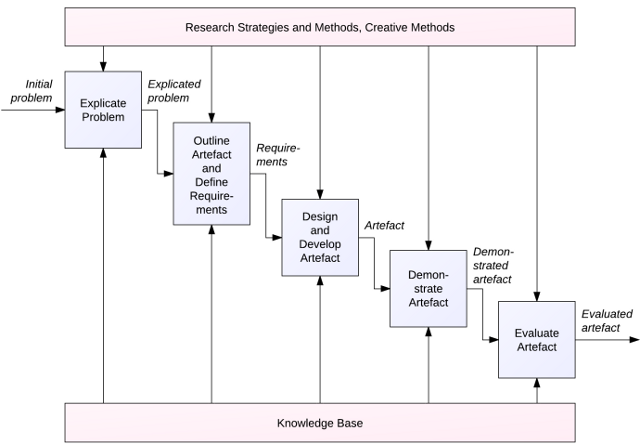
\includegraphics[scale=0.50]{part_3/design_science.png}
		\caption{Diagram of the Design Science Method \cite{johannesson2012design}} 
		\label{ds}
\end{figure}

The method chosen for this research is design science as defined by Johannesson and Perjons in A Design science primer \cite{johannesson2012design}. It is well structured and has guidelines that makes it easy to use as opposed to other definitions of design science such as the one laid out in Memorandum on design-oriented information systems research \cite{osterle2010memorandum} or the one mentioned in Design science in information systems research \cite{hevner2004design}. Johannesson and Perjons mention that Design Science consists of 5 actions, as shown in figure \ref{ds}. This actions not proposed to be used in a sequence, the steps should be used in an iterative way. In design science it is possible to use other methods to answer questions about artefact. Every action in Figure \ref{ds} should have its own methodology or it can even have several methodologies. MediaSense is still a research project and real life use cases would require applications and therefore the demonstration action will not be performed as it's not valuable to this research.

\section{Research Strategies and Methods}
\section{Research method for Explicate Problem}
To explicate the problem we chose to do a document study of previous publications regarding internet of things middleware. The document study also considered of reading the source code for MediaSense to get an insight into how MediaSense is constructed and how it worked. Combining this method with interviews of a person with more knowledge about the concept internet of things and knowledge about MediaSense helped to explicate the problem and give a broader knowledge base of the surrounding concepts for internet of things middleware. With a broader knowledge base the problem can then be broken down into a number of subproblems. 

An alternative to these methods could be survey using questionnaires, in which predefined written questions can be asked to a respondent. This method can easy be distributed to a large number of respondents. It was not chosen because the researcher cannot ask follow up questions which makes it hard to discuss a problem situation and because there are few persons with knowledge about MediaSense the result of a questionnaire would not explicate the problem, especially when follow up questions is not possible. If there was a larger group of stakeholders for MediaSense a survey could have been used to explicate the problem, but this was not the case and surveys was excluded.

\section{Research Method For Define Requirements}
Due to there only being one stakeholder with sufficient knowledge of MediaSense and as such quantitative methods are not applicable for defining the requirements of the artefact.
The qualitative methods we considered were observation, case study, interview and group discussions. To perform an observational study we would need a subject to observe in its natural environment but distributed Internet of Things middleware is still a subject of research and as such the intended environment does not yet exist. Conducting group discussions is not applicable in our situation because there only is one stakeholder.
Interviews at first seemed like a good approach because there only is one very involved stakeholder with whom we can conduct the interviews and thus get a deep understanding of the stakeholders needs. A problem with interviews is that the reliability or validity of the answers isn't guaranteed \cite{golafshani2003understanding}, even though the respondent might answer to their best ability it is possible that not all requirements are immediately unearthed due to the restricted perspectives. Interviews also tend to stifle creativity and are dependent on the questions asked \cite{johannesson2012design} thus resulting in important requirements being missed. Because the stakeholder also was responsible for the artefact the answers given in an interview could be coloured by his own view of the artefact.
A case study with both interviews and a deeper study of the artefact was then the best solution as this would make it possible to determine how aspects of the artefact worked before conducting unstructured and open-ended interviews to determine how the solution should work.


\section{Research For Design And Develop Artefact}
With the information gathered in the earlier stages of the design science process architectural changes will need to be designed. For this process participative modelling \cite{johannesson2012design} and document study will be used. The participative modelling will mainly be done by drawing architectural models on a whiteboard and the document studies will be done to research similar solutions and usable technologies. 

The development of the design will be done with pair programming \cite{williams2000all} which is a practice from the software development methodology extreme programming. According to  \cite{williams2000all} two programmers working together will find twice as many solutions to a problem than working alone. Also bugs will be found in an earlier state and this will give higher quality on the artefact. 

\subsection{Evaluate Artefact}
To evaluate the artifact it is necessary to validate that the requirements gathered in the earlier action \emph{defining requirements}, have been met. The strategies considered for evaluation are Surveys, Experiments, Case studies, Ethnography, Theoretical Analysis. 
Doing an ethnographic study would give valuable insights into how an Internet of Things platform would be used and how our redesign would impact usage. Given that Internet of Things still isn't a widely adopted paradigm there would be no precedent to compare cultural impacts to. Such a study would only contribute to the understanding of how people use the Internet of Things and not our artifact specifically. A case study allows for a deep study of the artefact but can be biased by the researchers perceptions, thus doing a case study of an artifact we ourselves developed will be inconclusive as to if the artifact fulfils the requirements.
Experiments allow us to set up an artificial scenario similar to that in the demonstration. The experiment will be designed to specifically validate all the requirements. A drawback to using experiments is that the artificial scenario doesn't reflect a real life scenario. To rectify this we will use Theoretical analysis of the results from the experiment. Thus we chose to evaluate the artifact with experiments and theoretical analysis.


\section{Ethical Considerations}
All information uncovered in the interviews will be used confidentially and we will assure the respondent consensually agree to have all answers published in this thesis.
The MediaSense platform uses the GNU Lesser General Public License, version 3 \cite{gnu} and as such, there is no confidentiality we need to observe regarding the source code of it.
All test environments used for testing the distributed Internet of Things middleware will be run on a local sandbox for development so the nodes in the network will only contain our own computers. 
    \chapter{Explicate Problem}
The explicate problem step in Design Science \cite{johannesson2012design} is to formulate precisely the initial problem and investigate its underlying causes. To define the problem as precisely as possible a scenario will be defined. The problem was split into several sub-problems. As mentioned before the research method for explicating the problem is a document study of previous publications regarding distributed Internet of Things middleware, document study of reading the source code for MediaSense and interviews with the lead developer of MediaSense. 

\subsection{Research Question}
As the authors discuss in \cite{johannesson2012design} a research question was formulated to form the basis of the problem explication. For the problem explication part of the project the research questions is the following: 

\begin{quotation}
What are the major issues with current implementations of distributed Internet of Things middleware which make them unable to realize the Internet of Things vision?
\end{quotation}

\subsection{Method Application}
To explicate the problem a document study of previous publications regarding distributed Internet of Things and middleware for it was done. Some of the publications regarding MediaSense were provided by the stakeholder \cite{TheMediaSenseFramework}, \cite{Kanter539187}, \cite{Walters413794}. These provide background on Internet of Things, what MediaSense is and how it works theoretically. Publications about Internet of Things and the surrounding theories were found by searching IEEE Xplore, ACM Digital library and Google Scholar. The main search queries used were \emph{Internet of Things}, \emph{Internet of Things middleware}, \emph{Internet of Things centralized} and \emph{Internet of Things decentralized}. Because the concept Internet of Things is a popular research area, a lot of articles was found. Publications was selected by reading the abstract to see if the publication were able to expand the knowledge base for the problem, searches for keywords were done and ranking publications after number of citations was done to narrow down the search result. 

After getting a grasp of the current state of Internet of Things middleware unstructured interviews were conducted with the stakeholder and main contributor to the MediaSense platform. This respondent has a lot of experience with distributed computing and a good understanding of how Internet of Things middlewares works, therefore this respondent was the best person to interview. The interviews were conducted in an informal manner in both the stakeholders office and in a conference room with access to a whiteboard. No recording or notes were done for the interviews thus availed both authors to be active in the interviews and discussions could be done without thinking of recording or taking notes. These interviews were conducted iteratively and in parallel with a document study of the existing source code of MediaSense. This document study yielded questions for upcoming interviews and the interviews in turn gave more information about the inner workings of Internet of Things middlewares and how to proceed the study of MediaSense's source code.

Interviews began with trying to discover the problematics of the chosen Internet of Things middleware. The stakeholder first presented a problem that had been identified with MediaSense, a large resource overhead when running multiple applications. The first set of interview questions served to fill the gaps that documentation normally would. The questions aimed to explore how MediaSense worked and to get a broader knowledge base. After studying the source code and getting an understanding of the architecture, the interview questions explored certain modules functionality and how they worked. When the interviewee responded to the questions in an uncertain manner, the follow up questions were formulated to ascertain how they were supposed to work or how it was intended they should work.

After the application of methods used to explicate the problem an analysis was done on the result from the interviews and the document study. This was done by putting together the result from the interviews and the knowledge that was built when the document study of code was done. By using the answers from the interviews and reproducing the problems mentioned by the respondent on a developer instance of MediaSense, the problem was clearer from a technical view.

\section{Results And Analysis}
The following scenario describes a use case scenario of an Internet of Things platform.

\subsection{Scenario}
Johan is CEO for a company in Stockholm. He is always on the move from meetings with his co-workers at work and to his daughter's football practice after work. His apartment is equipped with broadband and he has a Raspberry Pi computer connected to the Internet through a router. This Raspberry Pi is working as an information hub for Johan. The computer is running a distributed Internet of Things middleware and has 20 application installed. Johan has bought a new temperature regulator for his apartment. This regulator comes with an application that can be installed on his information hub. The temperature regulator is context-aware, it gets GPS information from Johans mobile phone and regulates the temperature in his apartment according to this. When he leaves home every morning the heating in the apartment turns down. At work Johan receive notifications to leave for meetings based on where the meetings are and how long it will take him to get there. When Johan leaves work his car's navigation system checks with his calendar if he has anything on his schedule, discovers his daughter has football practice and plots a course to the practice to pick her up. Johan's mobile phone alerts his heating regulator as he approaches his home and the heating is turned back on. Another application is connected to a thermometer by Johan's house and collects information about the temperature outdoors and adjusts the heating of according to this information.

\subsection{Define problem}
Distributed Internet of Things middlewares are resource heavy, which makes them inefficient to run on ubiquitous devices. Centralized Internet of Things middleware can solve this problem, but centralized approaches are more vulnerable and it can not be guaranteed that the server is always up and ready to respond to clients requests. Therefore, a distributed Internet of Things middleware needs to be redesigned to reduce the resource footprint. The chosen middleware for redesign is MediaSense. MediaSense is being developed by researchers at the Department of Computer and System Sciences at Stockholm University and is open source. 

After the interviews and document study of the source code of MediaSense the main reason for the resource overhead was identified. MediaSense in its present form makes it necessary to run the platform once for every application. Every application running on a device needs its own instance of the middleware. This makes it necessary to run a middleware for every application running on a device, which is the main reason of the resource overhead. 

\begin{figure}[h!]
		\centering
    	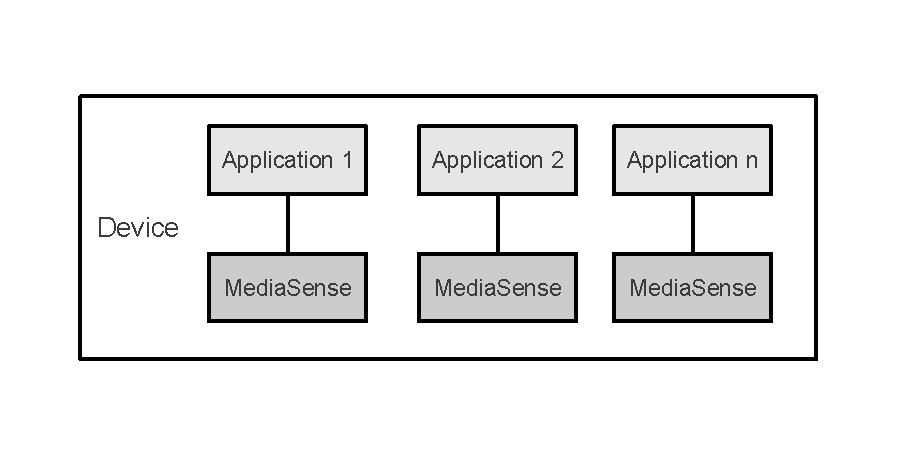
\includegraphics[scale=0.75]{part_4/result_and_analysis/mediasense_arch_old.pdf}
		\caption{The current state of the Mediasense platform showing how every application need its own instance of MediaSense.} 
\end{figure}

A sub-problem to the multiple middleware instances is that every instance need its own port for communicating. Because MediaSense is communicating over IP every instance needs its own port open. This means that a user needs to open new ports on the router and firewall for every application running on the device. When several instances of MediaSense is running on a device the network traffic increases, more processing power is used and more memory is used. 

\subsection{Motivation}
To make the scenario presented above possible an Internet of Things middleware it is needed to facilitate the communication between devices. Because the devices used in the scenario are mobile this middleware needs to be resource efficient. The devices need to handle a multitude of applications. Given the current state of MediaSense, the scenario will not be possible because of the resource overhead. To make the Internet of Things concept possible on ubiquitous devices this resource overhead must be dealt with.

\subsection{Analysis Of Problem}
With distributed Internet of Things middlewares every instance of the middleware is both a \emph{server} and a \emph{client}. Every instance of the middleware have its own network layer and database layer for storing context information. In a centralized middleware the server functionality can be moved to a centralized computer and therefore centralized middleware are more lightweight. This is one of the reasons distributed Internet of Things middleware are resource heavy. 

To reduce the resource overhead it is prefered to change the architecture of MediaSense. Changing the architecture so that only one shared instance of MediaSense is running can reduce the resource used on a device.  As shown in figure the desired architecture of MediaSense MediaSense will be run as an underlying  \emph{daemon} and every application needing the services from the platform can use the daemon. This also solves the subproblem with multiple network layers on one device. Devices only need one open port on router or firewall to communicate with other nodes in the network.  

\begin{figure}[h!]
	\centering
    	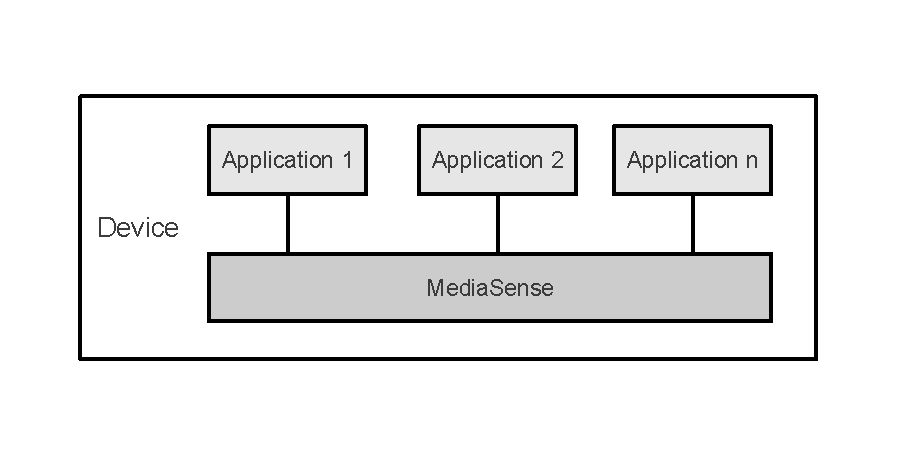
\includegraphics[scale=0.75]{part_4/result_and_analysis/mediasense_arch_new.pdf}
    	\centering
		\caption{The desired state of the Mediasense platform.} 
\end{figure}


    \chapter{Outline Artefact and Define Requirements}
This activity in design science involves identifying and outline an artefact that can address the explicated problem and also define requirements for the artefact \cite{johannesson2012design}. The requirements will help to get required functionality and constraints for the new artefact. 

\subsection{Research Question}
- Which architectural changes can be done to reduce the resource overhead of the chosen Internet of Things middleware?

- What are the requirements to make a distributed Internet of Things platform able to run on ubiquitous devices?


\subsection{Method Application}
The case study of MediaSense began by examining its architecture. The problem explication made it clear that the platform needed to be run as one separate instance and give applications an interface to communicate with it through. This required knowledge of what parts of MediaSense the applications had access to and deciding which parts of MediaSense should be shared between applications. Interviews with a stakeholder, the lead developer of MediaSense, was conducted to determine the requirements for the artefact. The interviews were connected to the case study where investigations of different scenarios were done. These were done in the form of informal open-ended interviews with the goal of understanding which the problems were with the old artefact and how the new artefact should work.
From the information collected from the case study and the open-ended discussions a list of requirements was extrapolated. This activity was done in an iterative way under the design and develop activity as new issues were detected. These issues were brought to the stakeholders attention and discussed in order to define new requirements. The MediaSense platform was profiled to obtain a benchmark for the memory consumption before our redesign.

\subsection{Outline Artefact}
To solve the problem a new type of Internet of Things middleware is required to be developed. Instead of developing a completely new middleware an existing one was chosen to be redesigned. The analysis of the problem explication uncovered that the main cause for the resource overhead in MediaSense is the distributed approach of the network layer. This is because every application has its own middleware and the middleware has its own server and client to communicate with other nodes. A redesign is necessary to build a middleware with one common instance of a middleware for every application. The new artefact is a fork of the existing middleware MediaSense. In \cite{johannesson2012design} four types of artefact is defined: \emph{constructs}, \emph{models}, \emph{methods} and \emph{instantiations}. 

\begin{quotation}
  \textbf{Constructs} are terms, notations, definitions, and concepts that are needed for formulating problems and their possible solutions.
  \textbf{Models} are used to depict or represent other objects.
  \textbf{Methods} express prescriptive knowledge by defining guidelines and processes for how to solve problems and achieve goals.
  \textbf{Instantiations} are working systems that can be used in a practice.
\end{quotation}
The artefact type will therefore be an instantiation.

\section{Results And Analysis}
This section shows the requirements found from the case study and interviews. Requirements are categorized in functional requirements and non-functional requirements \cite{Roman1985}. The requirements all pertain to the properties mentioned in \cite{johannesson2012design}. 

\subsection{Functional Requirements:}
\begin{description}
	\item[Several applications] \hfill \\
	One instance of the middleware should be able to handle several applications.
	This is requirement has the property modularity for allowing any combination of applications to use the platform simultaneously.
		
	
	\item[Interface to applications] \hfill \\
	Applications should be able to communicate with the middleware through an interface.
	This is a requirement with the properties flexibility and maintainability allowing the middleware to be changed without destroying compatibility with applications.
	
	\item[Platform as daemon] \hfill \\
	When several applications are running on one device one shared instance of MediaSense should be used for the applications. This can reduce the resource overhead and help solving the underlying problem with a resource heavy middleware. This requirement has an Interoperability property, which means that the artefact has the ability to work together with other artefacts \cite{johannesson2012design}. 
	
	\item[Common network layer] \hfill \\
	The case study showed that a lot of messages was sent from a platform to other platforms. If a common network layer could be used for all applications running on one device the network usages would decrease. With less network usage the battery of ubiquitous computers will have better battery time. This requirement has both the property of being efficient and modular. 
	
	\item[Application independent] \hfill \\
	Applications should be able to start and stop independently of the platform. A crashed application should not affect the execution of the middleware itself. This requirement has the property robustness which means that it have the ability to cope with failures, errors and other problems during execution \cite{johannesson2012design}.
	
	\item[Gateway] \hfill \\
	Run MediaSense platform on a gateway and applications on connected ubiquitous devices.
This requirement has the property accessibility because it allows for a greater variety of devices to use MediaSense. This requirement also has the property of efficiency because the connected ubiquitous devices will only need to run the applications.
	
	\item[Messages with scope] \hfill \\
	Messages to other MediaSense nodes should have a scope, either for a specific application or to all applications on the node. This requirement was added to maintain the coherence property of MediaSense. With several applications running on a node messages must be able to be sent to the specific applications.

	
\end{description}	

\subsection{Non-functional requirements:}
\begin{description}
	\item[Less Memory Usage] \hfill \\
	The redesign of MediaSense should use less memory so it is able to run multiple applications on ubiquitous devices. This requirement has the efficiency property.

	\item[Java Version] \hfill \\
	Because MediaSense was written using Java 1.5 the stakeholder would prefer if the redesign were done using the same version of java. This requirement makes the maintenance of the new artefact easy for the stakeholder. 
	
	\item[Object Oriented Style] \hfill \\
	The same object oriented style which had been used to write MediaSense should be adhered to. This requirement has the properties maintainability and elegance. When using objects as parameters for method calls only a few parameters need to be send, the objects can hold a lot of data that need to be used in the method. This is the code style the stakeholder prefers. 
	
	\item[Unmodified Overlay] \hfill \\
	The stakeholder preferred to not change the network layer of the old artefact. If possible, the network overlay module should be left unmodified. This requirement is to uphold the maintainability property.
\end{description}	




    \chapter{Design and Development}
This activity aims to design and develop the artefact that is going to solve the problem announced in the explicated problem. The artefact is based on the requirements gathered in the previous activity. This activity involves some document study and modelling to find the best design for the artefact.

%\section{Development Process}
Based on the requirements collected from the stakeholder it was clear that the chosen middleware, the MediaSense platform, needed to be split into two pieces. The resource heavy modules in the middleware should be able to run once on a device and several application should be able to use them. 

The way MediaSense worked meant an application was started together with the platform behaved as a single instance. Thus, the application had access to all of the platforms functionality. Splitting up the application and platform would mean the application would run as a separate instance and therefore not have access to the platforms methods, a means of communication would be needed between application and platform to make this functionality available. MediaSense is written in Java and Java programs are executed in Java Virtual Machines (JVM). This means that the platform would run in one JVM and then several applications can be started and communicate with the platform from their own JVMs. Because one of the requirements previously discovered was that applications should be able to run on other devices and use the platform as a gateway, this communication would need to work remotely over network.

A document study of Remote Procedure Call (RPC) implementations was initiated to decide how applications should communicate with the platform. By comparing the gathered information about different RPC implementations we decided on using Remote Method Invocation which is a Java specific RPC implementation. RMI supports sending entire Java objects as parameters which complies with the requirement of keeping the Object oriented style of MediaSense. It also forces all remote objects to throw RemoteExceptions which facilitates the Application Independent requirement because the platform can catch the exceptions thrown by applications and avoid going down with them. The main drawback with using RMI is that it is not as lightweight as other RPC implementations, but the resource overhead this causes is small in comparison to running several instances of the MediaSense platform.

To find the best way to change the architecture of MediaSense several participative modelling sessions were held where models of the old architecture were drawn on the whiteboard and changes was applied on these models to find the best solution to solve the problem.

\section{System Architecture}

\begin{figure}[h!]
	\centering
    	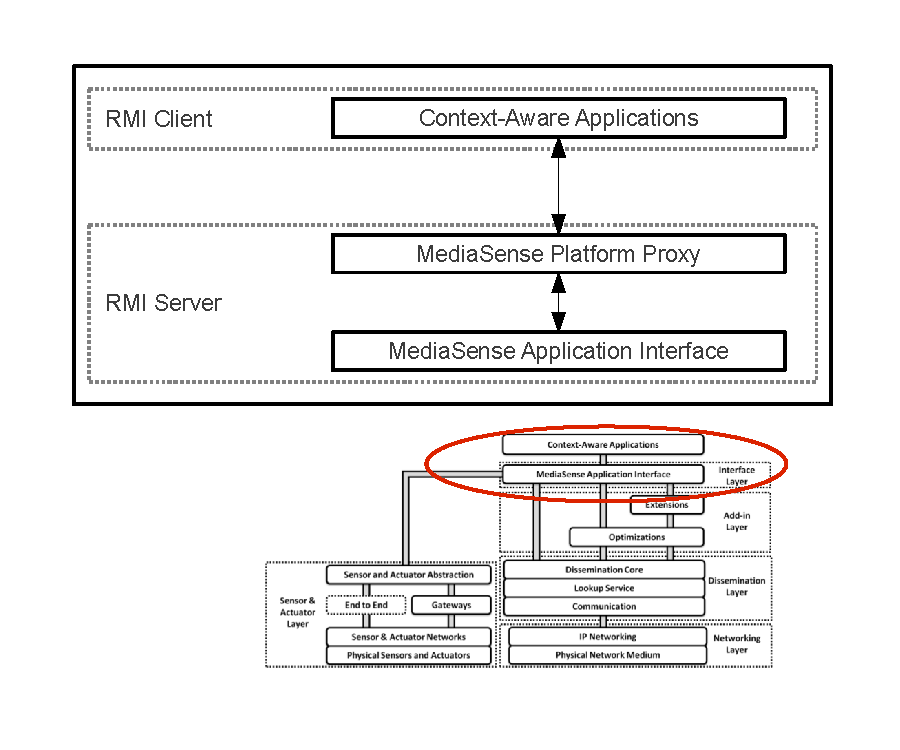
\includegraphics{part_6/artefact_description/changes.pdf}
		\caption{Figure showing how MediaSense Platfrom Proxy and application communicate with each other and where the RMI client and server is located in the architecture.} 
		\label{ds}
\end{figure}

\subsection{Network Overlay}
The network overlay handles the communication with other nodes and stores peer data in a database. The overlay has remained the same as in the old version of MediaSense and thus satisfies the requirement that the overlay should remain unmodified.

\subsection{MediaSense Messages}
MediaSense communicates with other nodes in the network by sending and receiving messages. Messages have a scope and can either be sent to a specific application or to all applications at a peer node. 
To create an application scoped message the application ID is sent as an argument to the constructor and the messages are then sent to the application that is identified with this ID. 
Messages can also be sent as peer messages, the message is sent to all applications on the receiving peer-node. In the original version of MediaSense, because every instance of the platform only ran one application, the messages had no scope and thus the applications would receive all messages. 
In the version that has been developed in this project, the dissemination core can redirect messages to specific applications. With the possibility to send messages to specific applications, the new version of MediaSense fulfills the requirement that applications should have scope.

\subsection{Dissemination Core}
The Dissemination layer in MediaSense includes different components, dissemination core and lookup service. The lookup service finds and resolves other entities who connects to the network. The dissemination core works as a router for the messages. When the platform is receiving messages the dissemination core handles these messages and sends them to the applications that are interested in those messages. If an application ID is specified, the message will be sent to the application with this ID. If the message type is set to be a peer message, the message will be sent to all applications connected to the platform instead. The dissemination core and the use of RMI satisfies the requirement that the artefact should handle several applications.

\subsection{MediaSense Platform Interface Layer}
The MediaSense Platform Interface Layer initiates the core components of the MediaSense platform, the Dissemination Core, the Pgrid lookupservice, and Pgrid's module for network communication. In the old version, it was also used to expose the functionality of the MediaSense Platform to the applications. In the new version, this component is only used by the RMI server. The client applications now access this functionality through the RMI Proxy which in turn calls the Interface Layer. This satisfies the requirement that applications should have an interface to the platform and that they should use a common network overlay.

\subsection{MediaSense Platform RMI Proxy}
This component is a RMI server that register itself to the RMI registry and makes it possible for RMI client to connect to it. The RMI proxy provides methods so the applications can communicate with the RMI server which is calling methods in the provided MediaSense Platform Interface Layer. The RMI server is acting as a shaded API so applications can call methods that are provided by MediaSense. This component makes it possible for several applications to connect to it and, therefore, only one MediaSense instance is needed for communication with the platform. This allows MediaSense to be run as a background process and thus satisfies the requirement that MediaSense should be able to run as a daemon.

\subsection{MediaSense Application Interface}
The application interface is used when a developer is developing an application. The developer extends this interface to get access to functionality that is needed for applications running on MediaSense. 
To create a MediaSense application, a few things are required. 

\begin{itemize}
  \item An application extending the interface must define its own unique application ID. This ID can be used to set the scope of a message to a specific application. 
  \item Applications must register what types of messages they are interested in receiving using the RMI Proxy's registerListener method. 
  \item An application needs to register itself on the platform by sending a reference of itself to be stored in the platforms list of applications. This is done by providing the applications ID as a parameter to the method called registerApplication in MediaSense Platform RMI proxy.
  \item The application interface contains one method that developers need to override, called handleMessage. This method is used for handling incoming messages to the application and responsible for responding to these messages. 
\end{itemize}

To communicate with the MediaSense platform, an application must first know the IP address of the device where the RMI registry is located. If the platform runs on the same device as the applications, an arbitrary port is used. After connecting to the registry, the RMI Proxy is located through a lookup on the registered name \emph{mediasense} and an instance of it is saved in the application. When the application interface needs to communicate with the platform a method called getPlatformInterface is available which returns the instance of the RMI Proxy, on which all calls to the platform then can be done.


    \chapter{Evaluation Artefact}
This activity is for evaluating the artefact, addressing both the defined requirements and the explicated problem. This activity shows if the designed and developed artefact solves the problem and shows how the evaluation of the artefact was done. 

%\section{Research Question}
\begin{quotation}
How has the redesign of MediaSense affected the resource consumption and does it fulfil the requirements?
\end{quotation}


%\section{Method Application}
The research strategy used to evaluate the artefact was an experiment. The experiment was done by running an instance of the artefact and measure the memory usage while it is running. First the platform was started to see how much resources the platform use. When the platform was connected to the network, the researchers started to connect applications to the platform and take notes of how much memory every application was using. To test the old version of the middleware a node farm was used. A bash script was used to start several applications where every application had its own MediaSense platform. 

When four applications had been started and connected to the platform a pattern in the resource usage was found. The data was then compared to data from the old artefact were an analysis was done to see if the new version use less memory resources. To see if all requirements were fulfilled different tests were done where every test had an expected result. All results were discussed between the researchers to address if the result was as expected and if the requirements had been met. 

The experiment was done on an PC with operating system Ubuntu 12.04.2 LTS. The computer in use has an Intel Core i3-2350M processor and 8 GB Memory. To measure the resources the applications Gnome System Monitor 3.4.1 \cite{gnomesm} and htop 1.0.1 \cite{htop} was used.

The non-functional requirements were not evaluated with a specific approach, they were discussed as the experiments took place to see that they were addressed and met. To measure if the new artefact consumed less of the devices memory one to four applications were run with both the old version of the middleware and the reengineered version. The results were noted and a comparison was then done. A test where the platform and the application ran on separate devices was also done to validate the Gateway requirement.

\section{Test Results}
\subsection{Functionality}

\begin{table}[!h]
    \begin{tabular}{ | l | p{12cm} |}
    \hline
    Test 	 				& 		 Start the platform\\ \hline
	Produce  				& 		 This was tested by adding the platform as a startup service on a linux computer. When the computer was started the platform started.\\ \hline
	Expected Results  		& 		 The expected result is that the platform starts and connects to the network without any applications connected to it. \\ \hline
	Results 				& 		 As Expected\\ \hline
	Comments				& 		 This test shows that the requirement Platform as Daemon is met.\\ \hline
    \end{tabular}
    \caption{Start The Platform}
\end{table}

\begin{table}[!h]
    \begin{tabular}{ | l | p{12cm} |}
    \hline
    Test 	 				& 		 Connect an application to the platform \\ \hline
	Produce  				& 		 This was done by starting a MediaSense application and connecting it to the background process from the previous test. The application registers itself with the platform and a connection to the platform is established. To see that the platform and the application is connected to each other the method getLocalhost() was called and the application printed this out in the output console. \\ \hline
	Expected Results  		& 		 The application connects to the platform and when the application register itself to the platform they are connected. When getLocalhost() is called the localhost for the platform should be printed in console. \\ \hline
	Results 				& 		 As Expected\\ \hline
	Comments				& 		 This shows that the old functionality still exists and work in the new artefact.\\ \hline
    \end{tabular}
    \caption{Connect An Application}
\end{table}

\begin{table}[!h]
    \begin{tabular}{ | l | p{12cm} |}
    \hline
    Test 	 				& 		 Connect several applications to the platform\\ \hline
	Produce  				& 		 Ten applications were connected to the MediaSense daemon. All applications register themselves at the platform using the Interface method registerApplication.\\ \hline
	Expected Results  		& 		 All applications connects to the platform and connections are established without any errors.\\ \hline
	Results 				& 		 As Expected\\ \hline
	Comments				& 		 This test shows that several applications can connect to the platform. This test also shows that the requirement \emph{Several Applications} is met.\\ \hline
    \end{tabular}
    \caption{Connect Several Application}
\end{table}

\begin{table}[!h]
    \begin{tabular}{ | l | p{12cm} |}
    \hline
    Test 	 				& 		 Storing an UCI\\ \hline
	Produce  				& 		 One of the applications connected to the platform store an UCI by calling the method registerUCI.\\ \hline
	Expected Results  		& 		 A DuplicateUCICheckMessage is sent from the platform and a DuplicateUCICheckResponseMessage will be received when the UCI is stored in the network.\\ \hline
	Results 				& 		 As Expected\\ \hline
	Comments				& 		 This test shows that the functionality still works. The methods which are called are from the provided Interface. This shows that requirement \emph{Interface to applications} is met.\\ \hline
    \end{tabular}
    \caption{Storing An UCI}
\end{table}

\begin{table}[!h]
    \begin{tabular}{ | l | p{12cm} |}
    \hline
    Test 	 				& 		 Resolving an UCI\\ \hline
	Produce  				& 		 An application connected to the platform sends a ResolveMessage.\\ \hline
	Expected Results  		& 		 The application should call the method resolveUCI, causing the platform to send a ResolveMessage. When the message has been routed through the network a ResolveResponsMessage should be received by the platform and be passed to the application. \\ \hline
	Results 				& 		 As Expected\\ \hline
	Comments				& 		 The methods that are called are the methods from the provided Interface. This shows that requirement \emph{Interface to applications} is met.\\ \hline
    \end{tabular}
    \caption{Resolving An UCI}
\end{table}

\begin{table}[!h]
    \begin{tabular}{ | l | p{12cm} |}
    \hline
    Test 	 				& 		 Sending a message\\ \hline
	Produce  				& 		 This was tested by building an application that sends NotifyMessages in response to a GetMessage. One of the connected applications sends a GetMessage and the application receiving this messages responds with a NotifyMessage.\\ \hline
	Expected Results  		& 		 A NotifyMessage should be received by the application that sent the GetMessage.\\ \hline
	Results 				& 		 As Expected\\ \hline
	Comments				& 		 The methods that are called are the methods from the provided Interface. This shows that the requirement \emph{Interface to applications} is met. \\ \hline
    \end{tabular}
    \caption{Sending Message}
\end{table}

\begin{table}[!h]
    \begin{tabular}{ | l | p{12cm} |}
    \hline
    Test 	 				& 		 Application crash with several application connected to platform\\ \hline
	Produce  				& 		 Connect several applications to a platform on one device. Make one of the applications crash by throwing an exception. A peer message was then sent to all applications connected to the platform.\\ \hline
	Expected Results  		& 		 Platform should still be working. No other applications connected to the platform should be affected by the crash. Messages should still be able to be sent and received by the platform.\\ \hline
	Results 				& 		 As Expected\\ \hline
	Comments				& 		 This shows that the requirement \emph{Application independent} is met.\\ \hline
    \end{tabular}
    \caption{Application Crash}
\end{table}

\begin{table}[!h]
    \begin{tabular}{ | l | p{12cm} |}
    \hline
    Test 	 				& 		 Send peer scope message\\ \hline
	Produce  				& 		 Sending a NotifyMessage from an application with the scope PEER. \\ \hline
	Expected Results  		& 		 All applications on the receiving node should get this NotifyMessage.\\ \hline
	Results 				& 		 As Expected\\ \hline
	Comments				& 		 Requirement \emph{Message with scope} is met.\\ \hline
    \end{tabular}
    \caption{Send Peer Message}
\end{table}

\begin{table}[!h]
    \begin{tabular}{ | l | p{12cm} |}
    \hline
    Test 	 				& 		 Send application scope message\\ \hline
	Produce  				& 		 Sending a NotifyMessage from an application with the scope APPLICATION and the application ID as an argument. \\ \hline
	Expected Results  		& 		 Application with the specific ID should get the notifyMessage. \\ \hline
	Results 				& 		 As Expected\\ \hline
	Comments				& 		 Requirement \emph{Message with scope} is met.\\ \hline
    \end{tabular}
    \caption{Send Application Message}
\end{table}

\begin{table}[!h]
    \begin{tabular}{ | l | p{12cm} |}
    \hline
    Test 	 				& 		 Connect an application to an external MediaSense platform\\ \hline
	Produce  				& 		 The platform was started on one computer and an application running on another computer connects to the platform by getting its reference from the RMI registry.\\ \hline
	Expected Results  		& 		 Applications can communicate with the platform running on a PC. \\ \hline
	Results 				& 		 As Expected\\ \hline
	Comments				& 		 Requirement gateway is met. \\ \hline
    \end{tabular}
    \caption{Connect Application To An External Platform}
\end{table}
\clearpage


\subsection{Resource Usage Measurement}

\subsubsection{Memory Usage Of MediaSense}
\begin{table}[H]
\begin{center}
    \begin{tabular}[t!]{ | l | l | l |}
    \hline
    Number Of Applications								& Memory Usage Old Version				& Memory Usage New Version\\ \hline
    0 													& 0 MB									& 66 MB\\ \hline
    1 													& 70.4 MB								& 86.2 MB\\ \hline
    2 													& 139.2 MB								& 104.4 MB\\ \hline
    3 													& 213.04 MB								& 123.6 MB\\ \hline
    4 													& 286.5 MB								& 141.5 MB\\ \hline
    5 													& 360.2 MB								& 161.7 MB\\ \hline
    6 													& 430.3 MB								& 182.7 MB\\ \hline
    7 													& 505.3 MB								& 202.4 MB\\ \hline
    8 													& 574.1 MB								& 223.7 MB\\ \hline
    9 													& 648.3 MB								& 242.6 MB\\ \hline
    10 													& 718.3 MB								& 262.9 MB\\ \hline
    \end{tabular}
    \caption{Showing how much memory MediaSense is using}
\end{center}
\end{table}


\clearpage
\begin{figure}[H]
		\centering
    	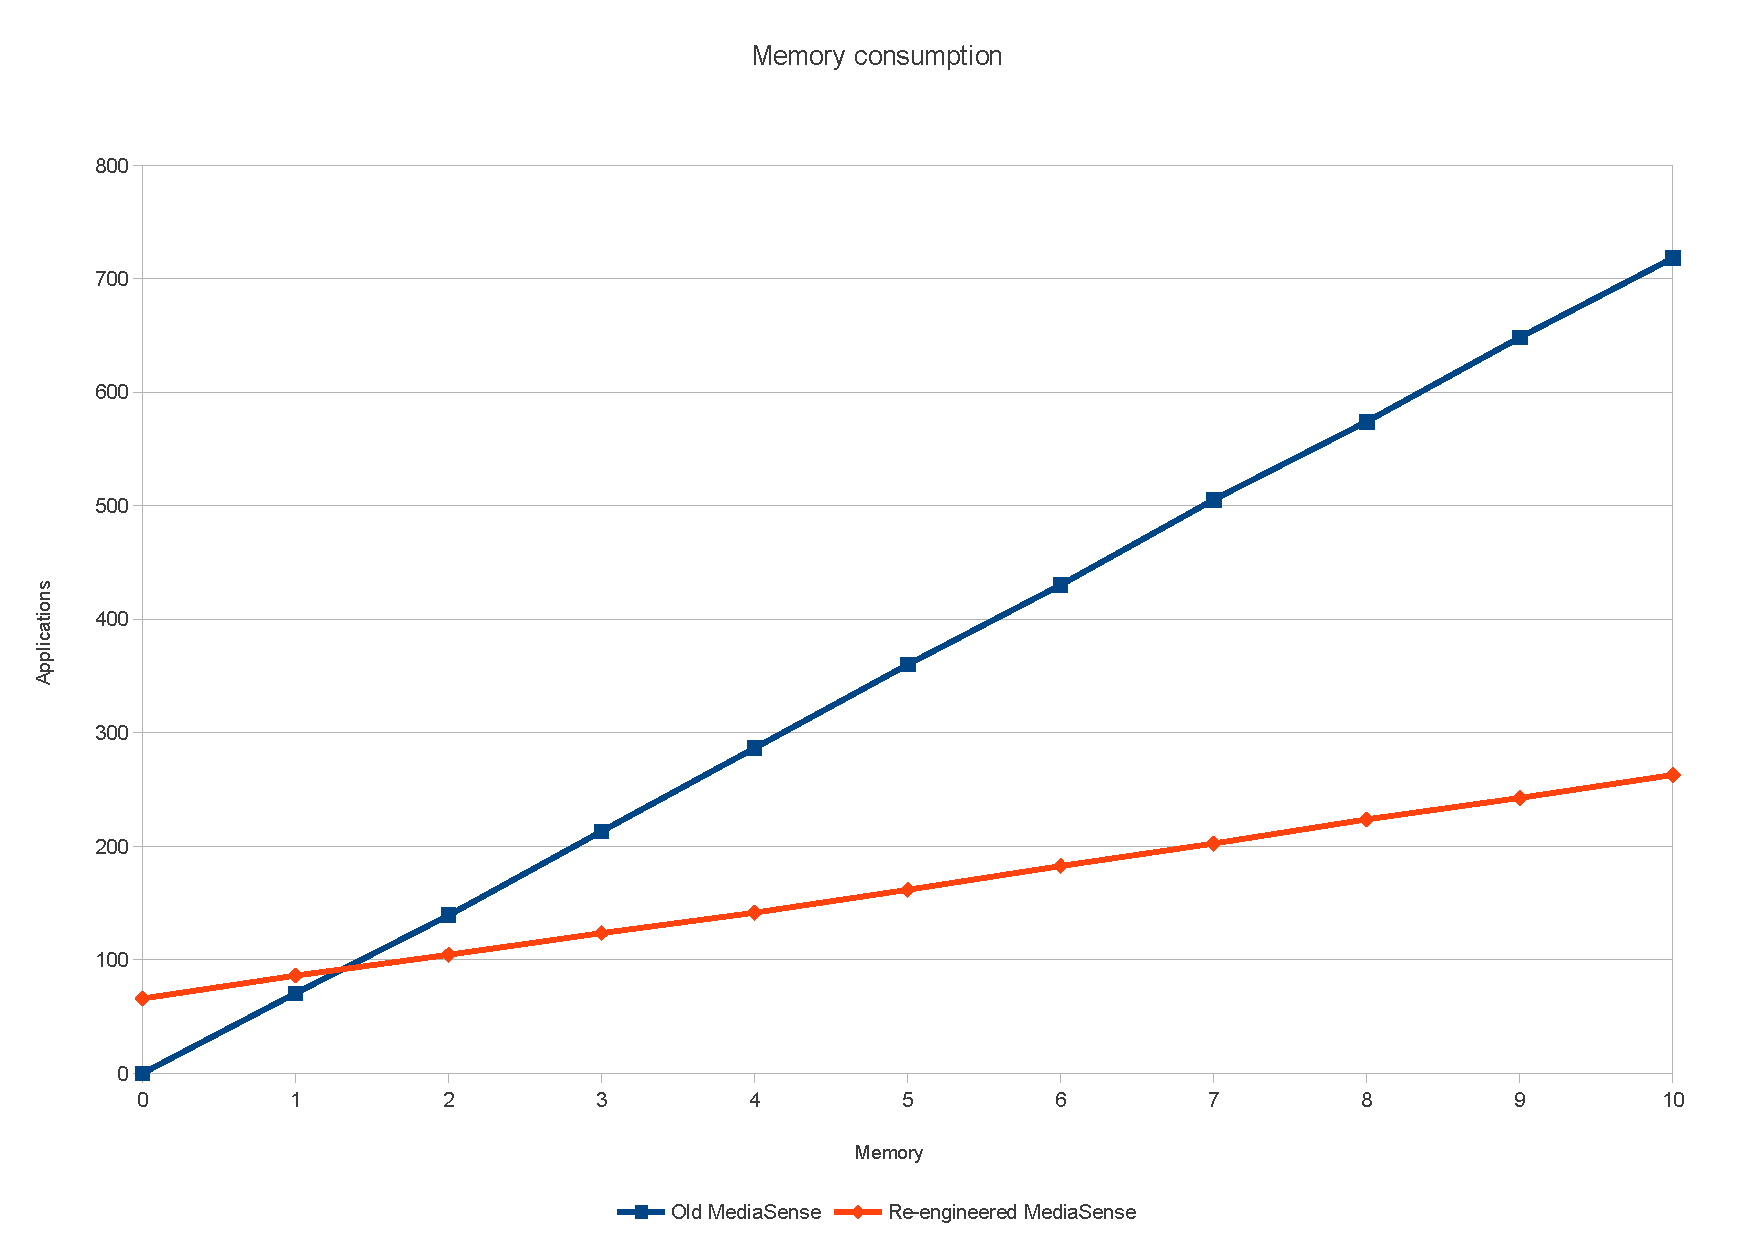
\includegraphics[scale=0.50]{part_7/test_results/memory.pdf}
    	\caption{Showing how much memory MediaSense is using}
    	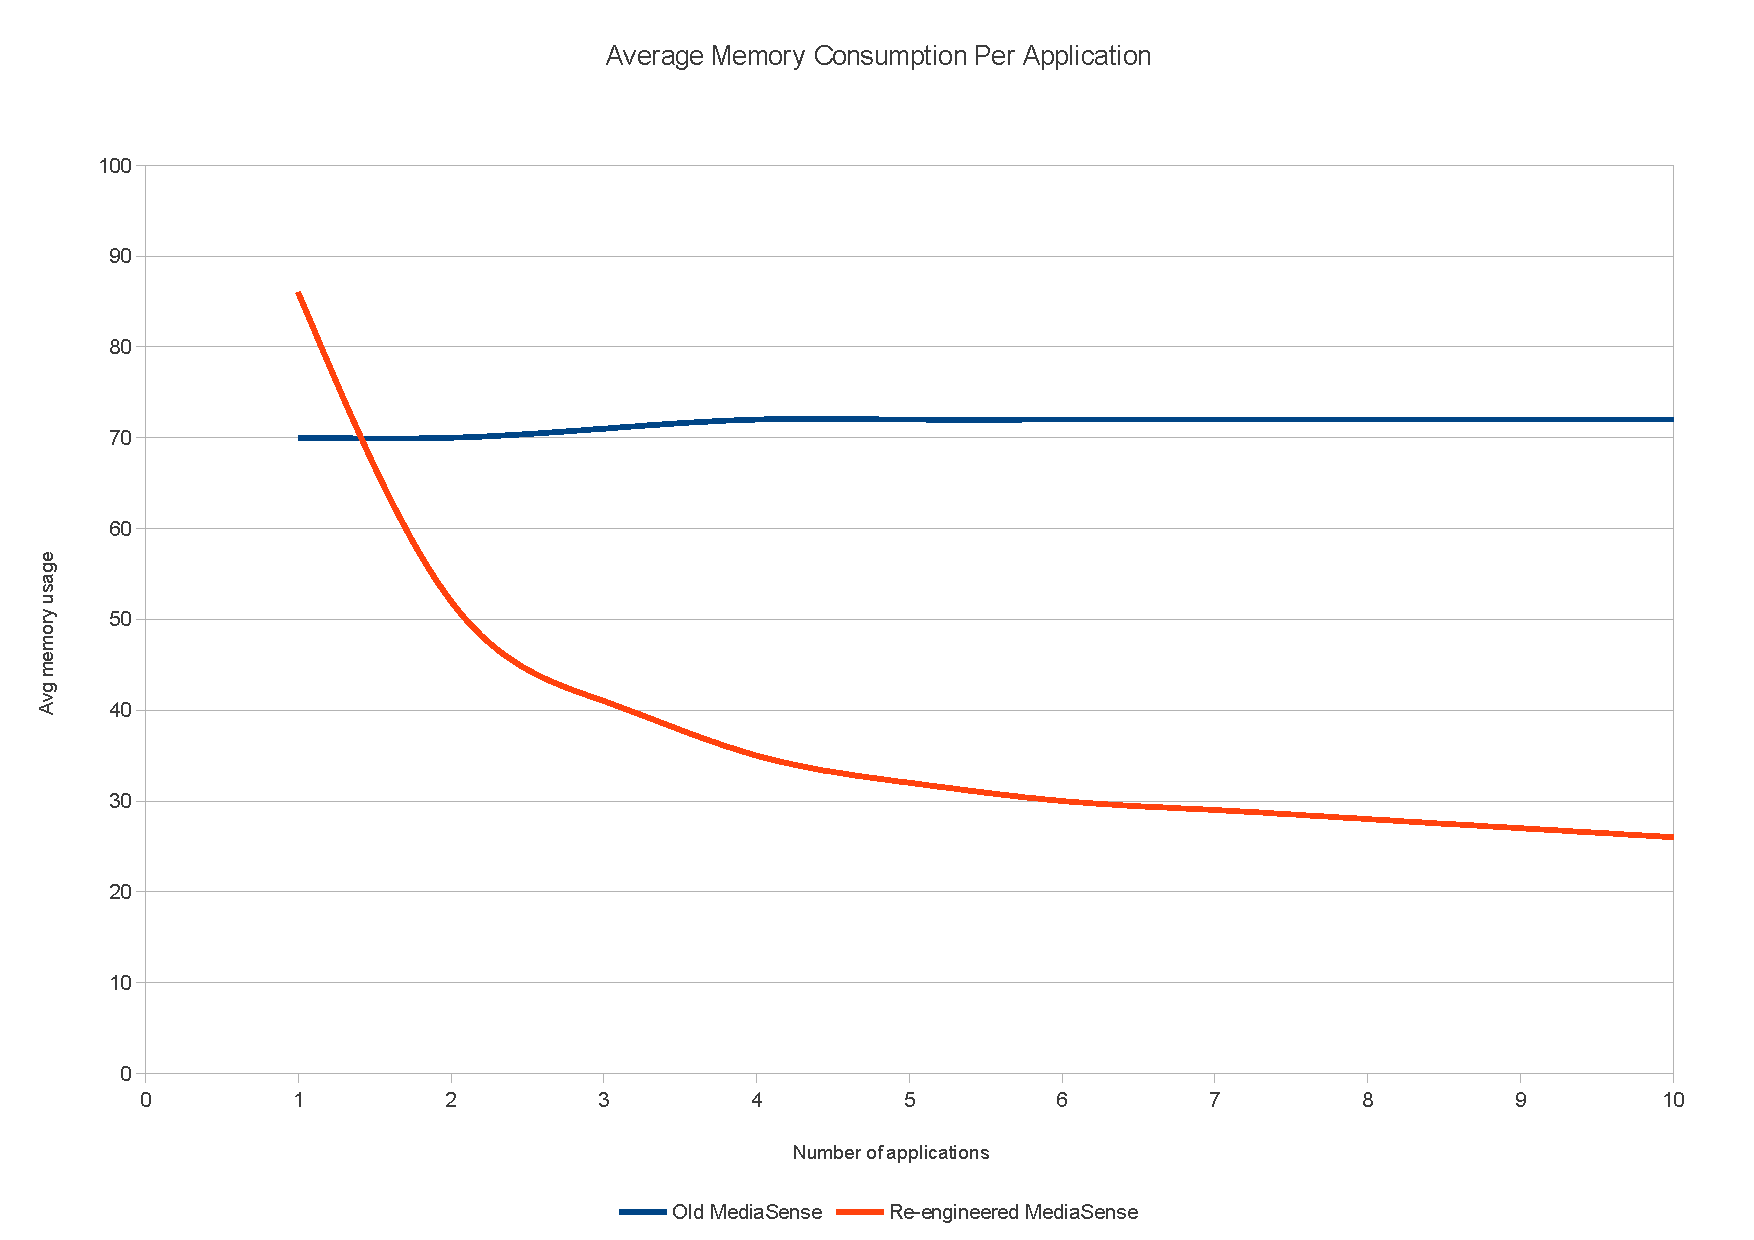
\includegraphics[scale=0.50]{part_7/test_results/avg_memory.pdf}
    	\caption{Average memory used by MediaSense per application}
\end{figure}


% ------------------------------

\subsubsection{CPU Time Of MediaSense}
\begin{table}[H]
\begin{center}
    \begin{tabular}[t!]{ | l | l | l |}
    \hline
    Number Of Applications								& CPU Time Old Version					& CPU Time New Version\\ \hline
    1 													& 2.70									& 4.21\\ \hline
    2 													& 5.34									& 4.57\\ \hline
    3 													& 8.72									& 6.2\\ \hline
    4 													& 12.88									& 8.12\\ \hline
    5 													& 15.43									& 9.23\\ \hline
    6 													& 18.82									& 9.60\\ \hline
    7 													& 21.58									& 10.67\\ \hline
    8 													& 24.85									& 11.96\\ \hline
    9 													& 27.84									& 12.88	\\ \hline
    10 													& 31.25									& 13.35\\ \hline
    \end{tabular}
    \caption{Showing how much CPU time MediaSense is using}
\end{center}
\end{table}
\clearpage

\begin{figure}[H]
		\centering
    	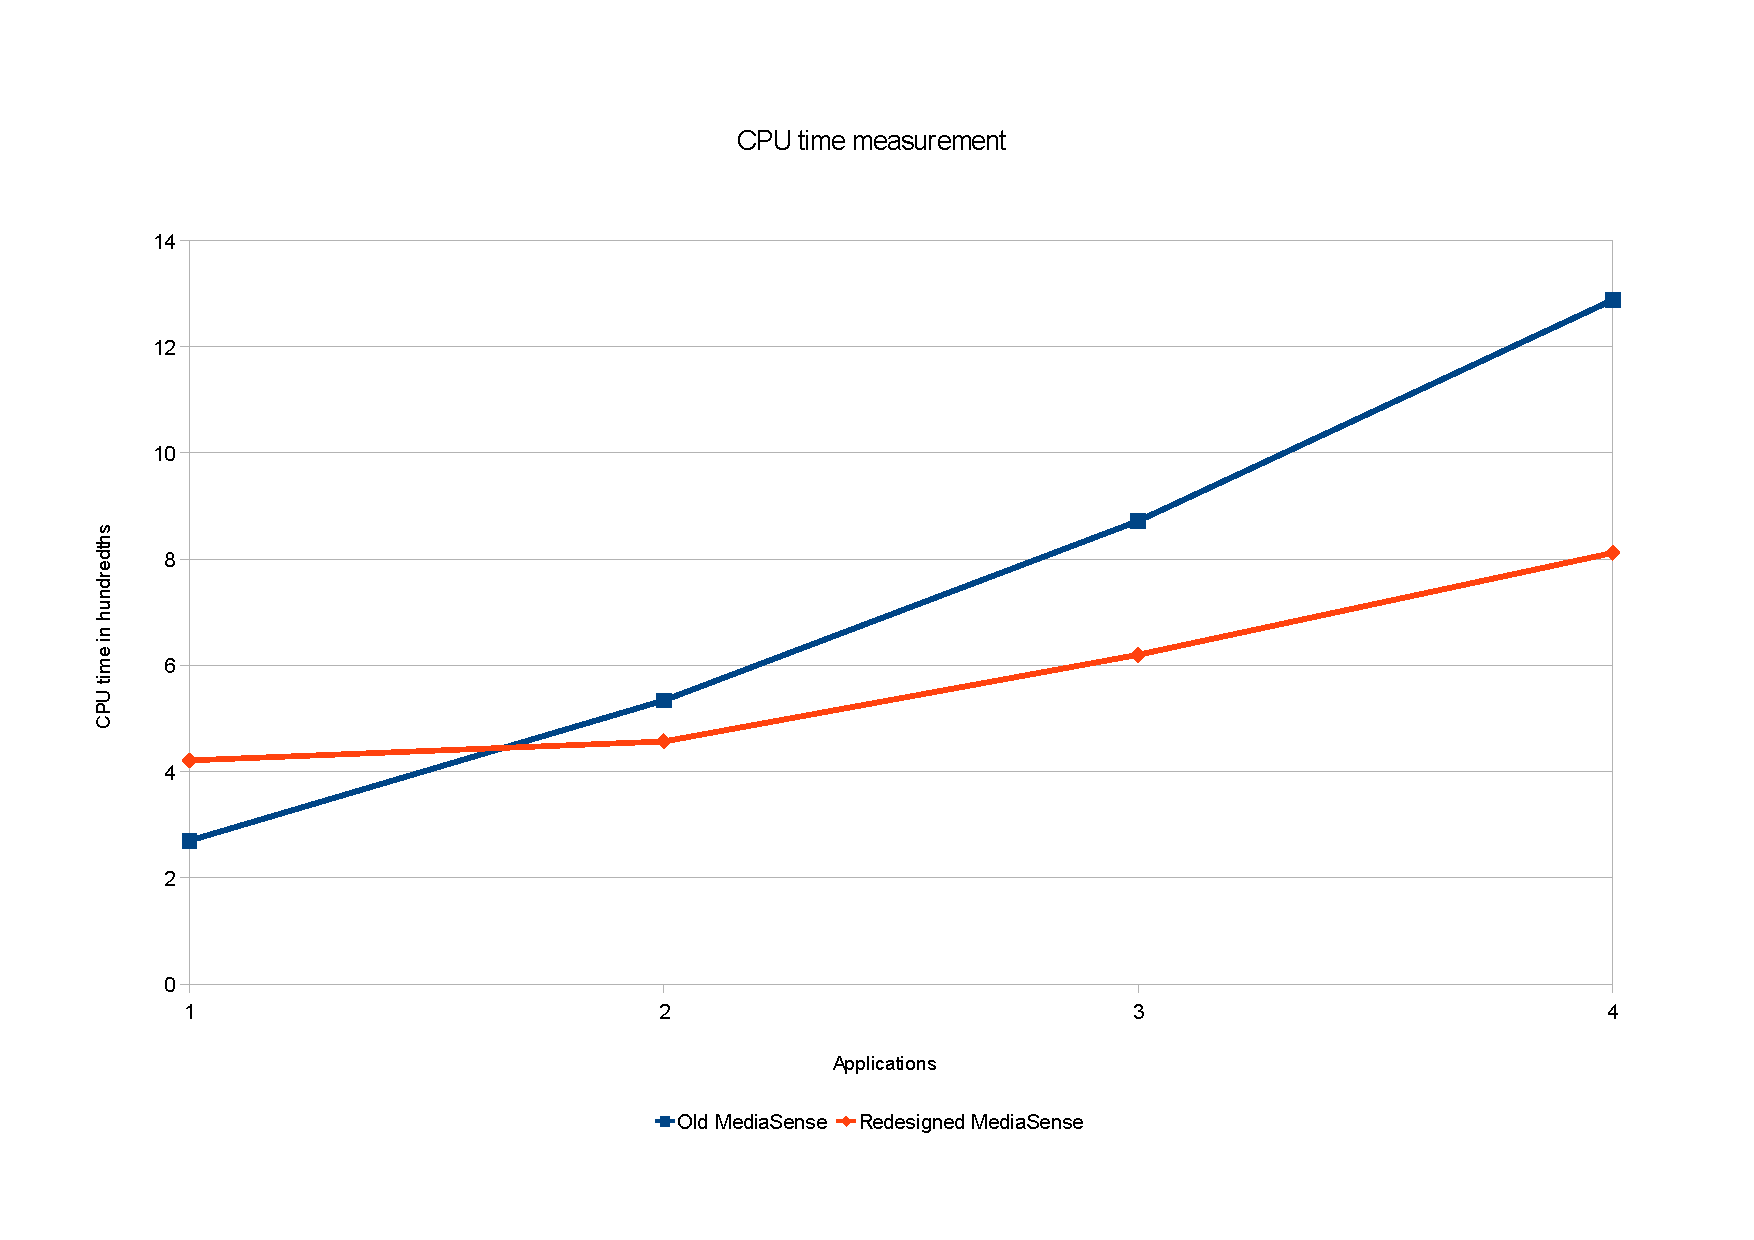
\includegraphics[scale=0.50]{part_7/test_results/cputime.pdf}
    	\caption{Showing how much CPU time MediaSense is using}
    	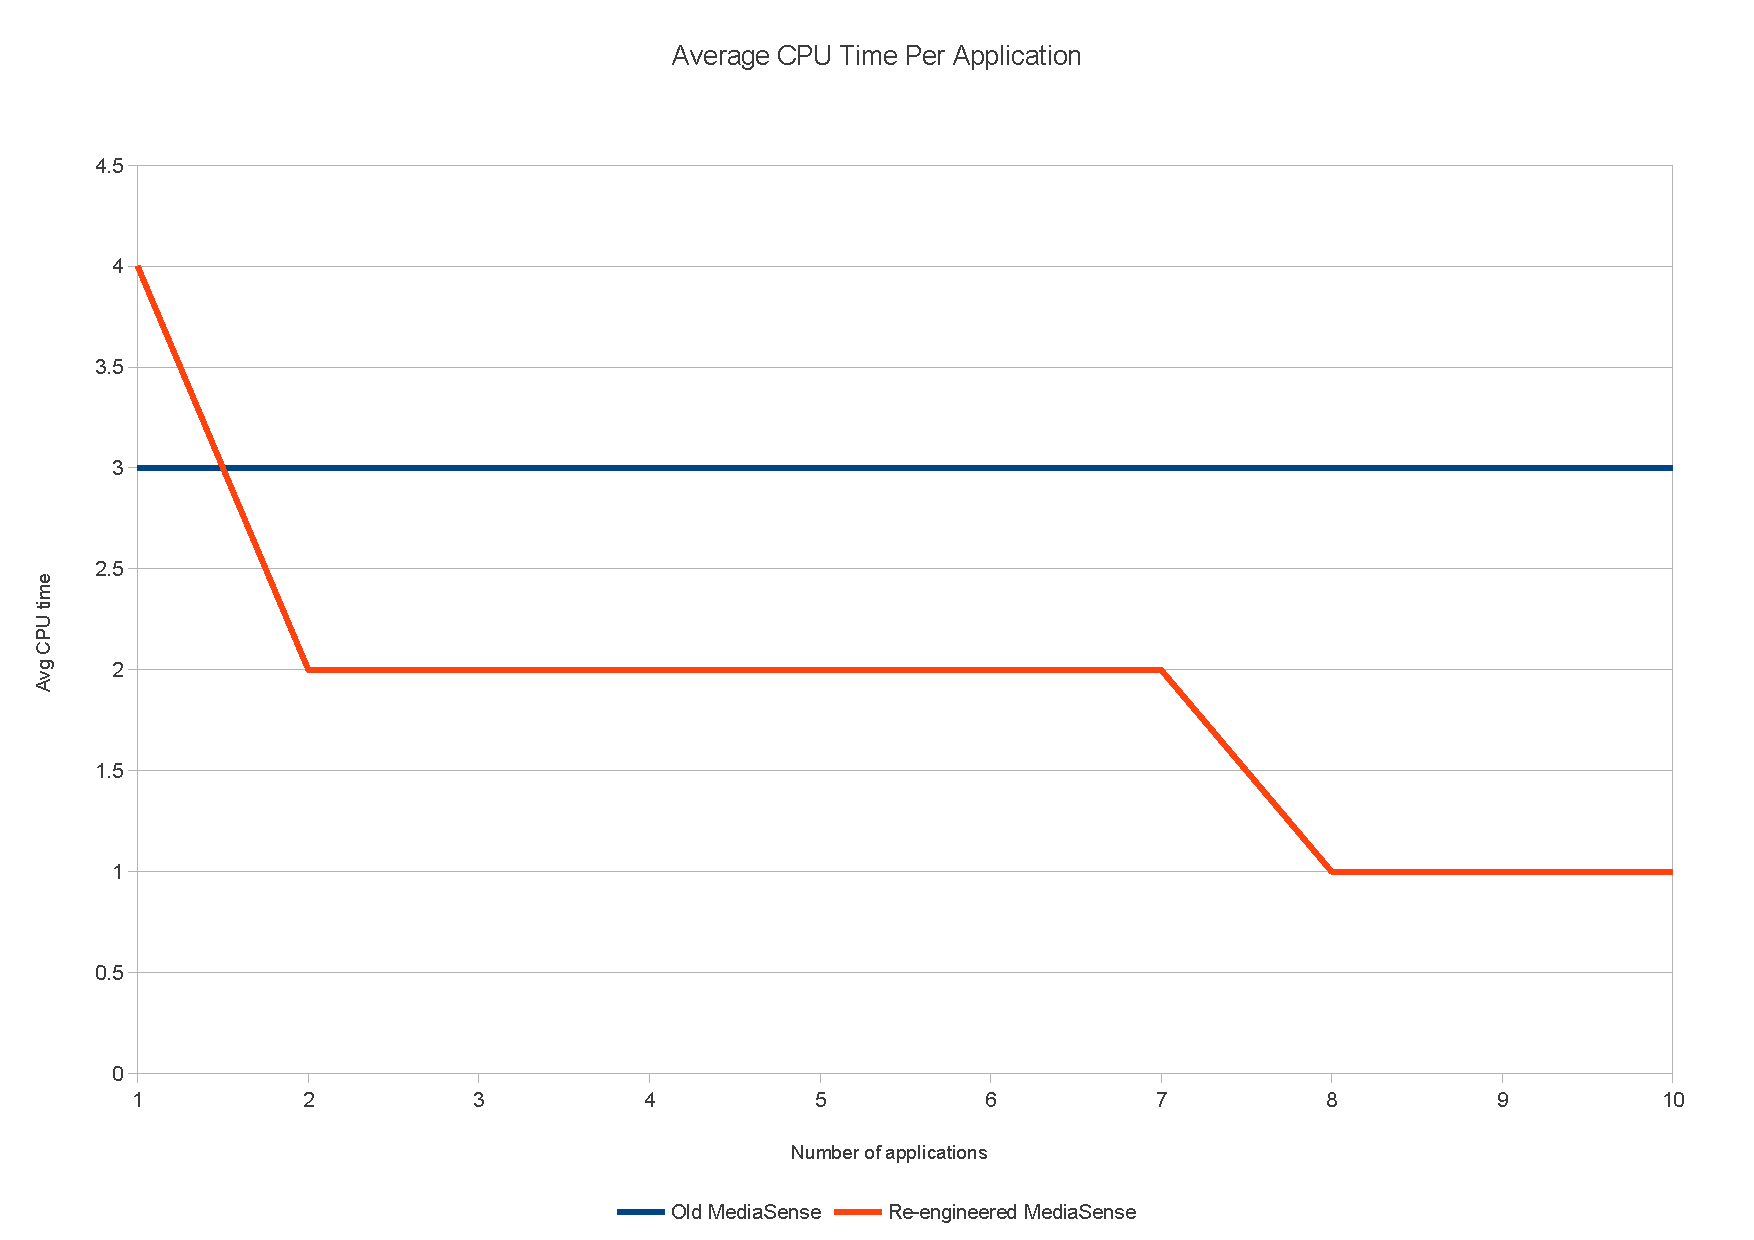
\includegraphics[scale=0.50]{part_7/test_results/avg_cputime.pdf}
    	\caption{Average CPU time per application used when MediaSense is running}
\end{figure}


% ------------------------------

\subsubsection{Threads Usage Of MediaSense Version}
\begin{table}[H]
\begin{center}
    \begin{tabular}[t!]{ | l | l | l |}
    \hline
    Number Of Applications								& Threads Old Version			& Threads New Version\\ \hline
    1 													& 30							& 55\\ \hline
    2 													& 60							& 75\\ \hline
    3 													& 90							& 95\\ \hline
    4 													& 120							& 115\\ \hline
    5 													& 150							& 135\\ \hline
    6 													& 180							& 155\\ \hline
    7 													& 210							& 175\\ \hline
    8 													& 240							& 195\\ \hline
    9 													& 270							& 215\\ \hline
    10 													& 300							& 235\\ \hline
    \end{tabular}
    \caption{Showing how many threads MediaSense is using}
\end{center}
\end{table}
\clearpage

\begin{figure}[H]
		\centering
    	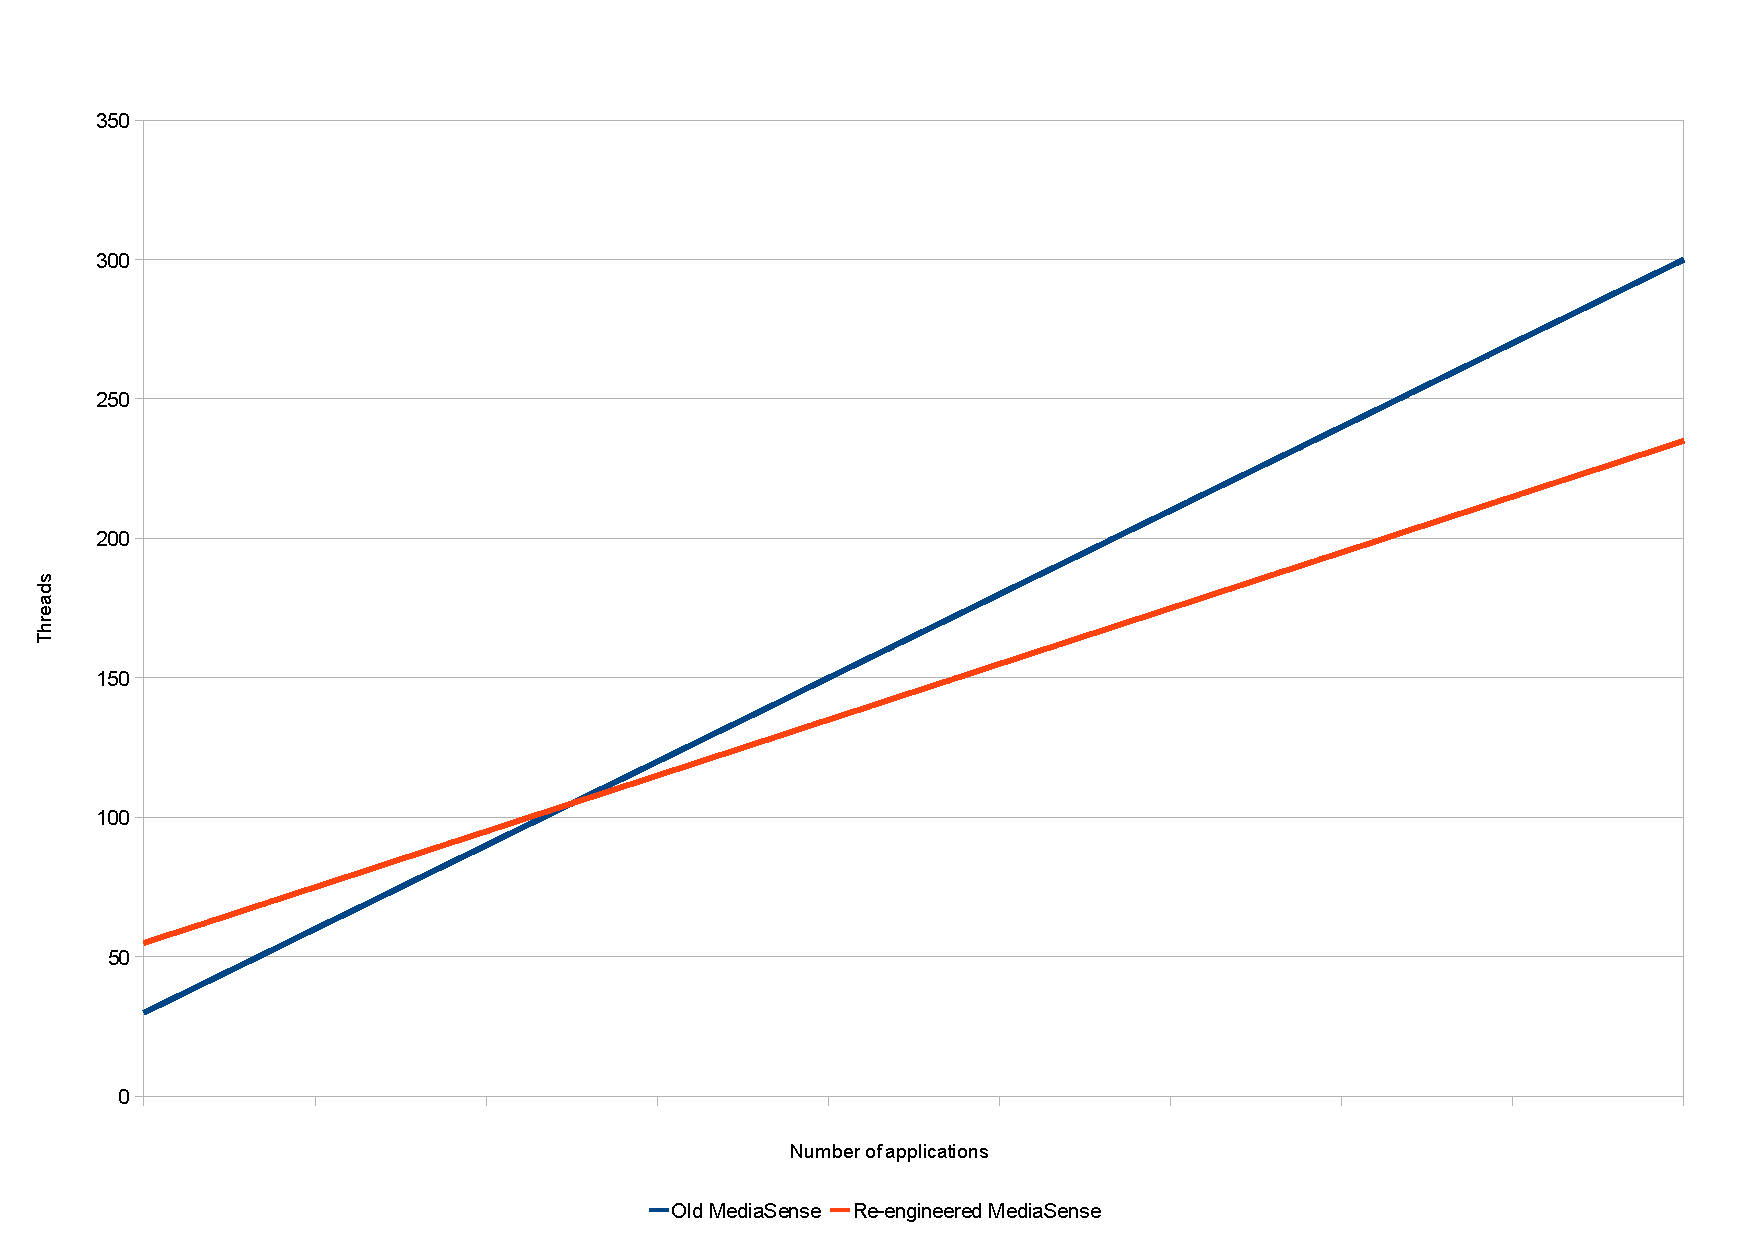
\includegraphics[scale=0.50]{part_7/test_results/threads.pdf}
    	\caption{Showing how many threads MediaSense is using}
    	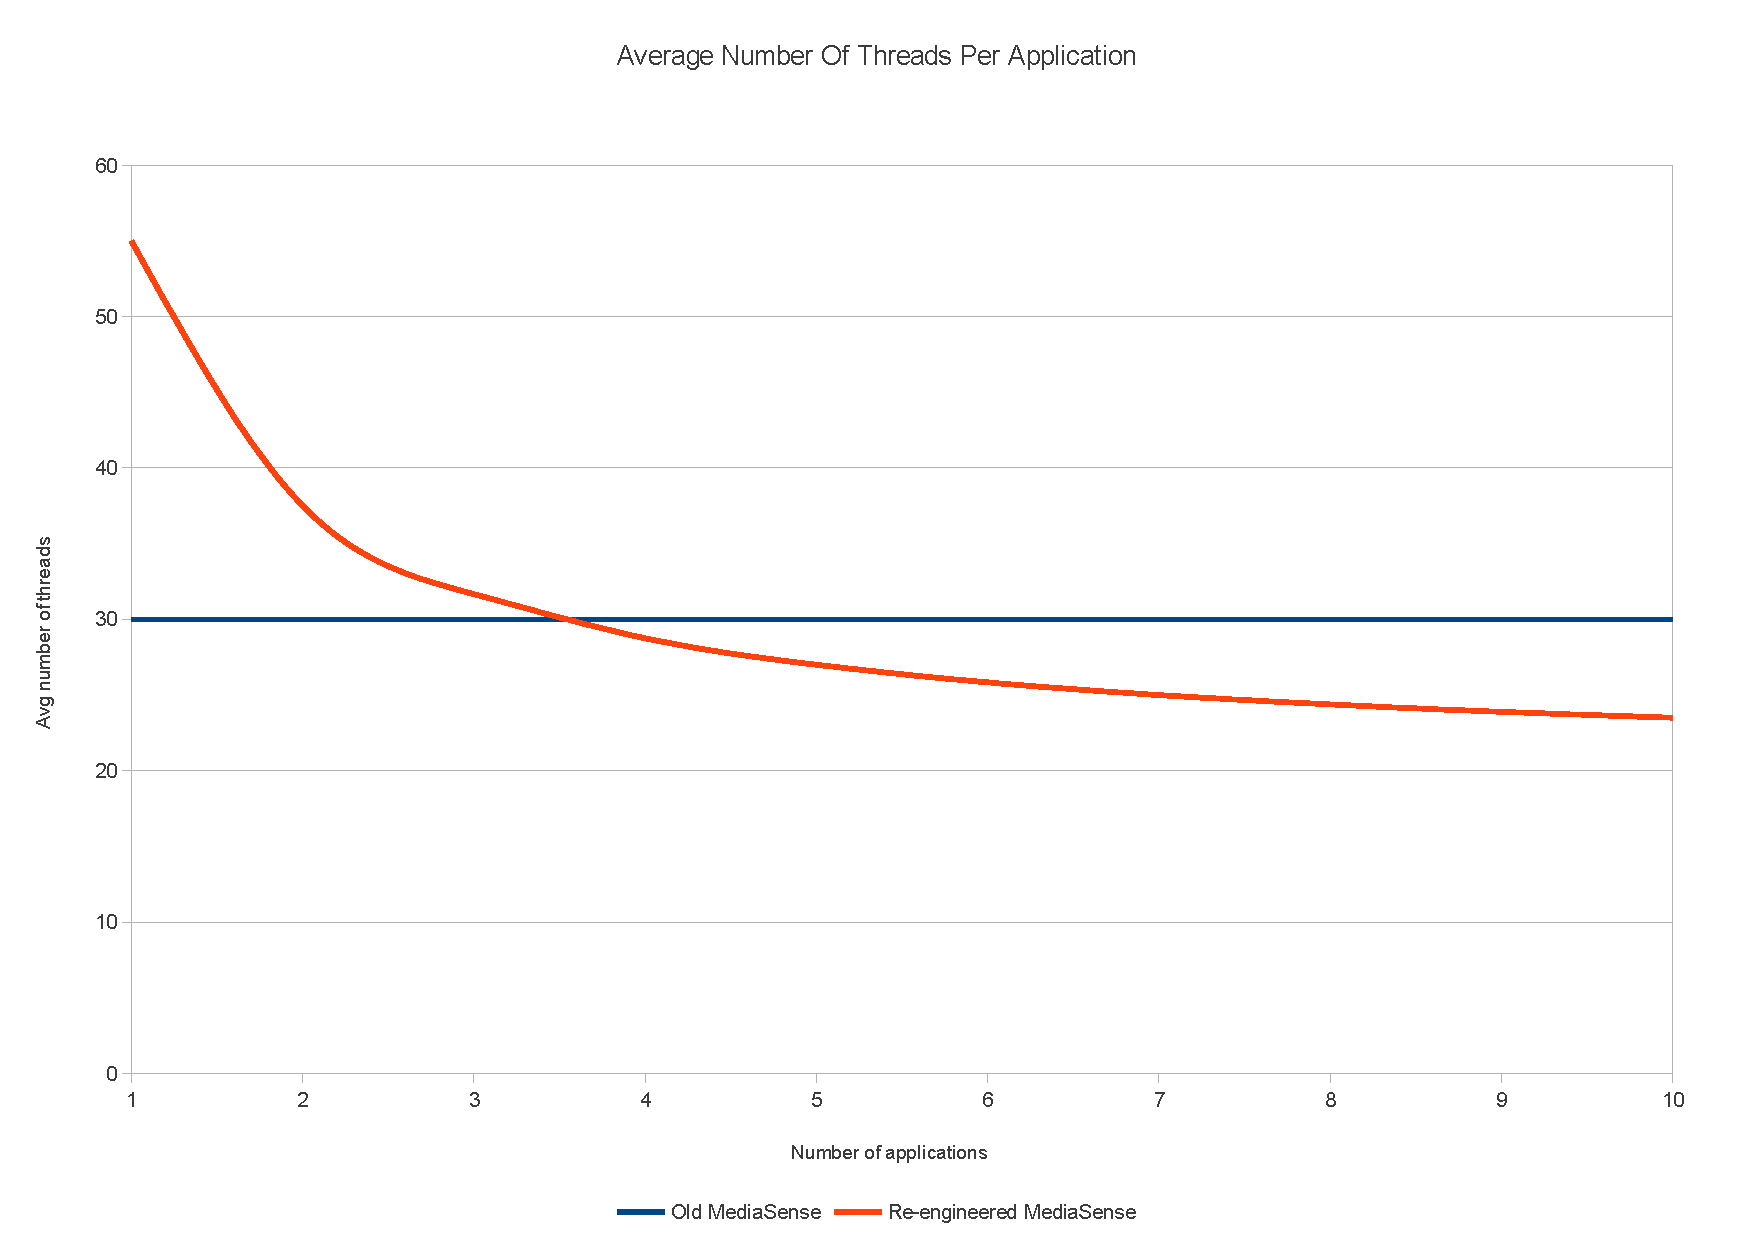
\includegraphics[scale=0.50]{part_7/test_results/avg_threads.pdf}
    	\caption{Average number of threads per application used when MediaSense is running}
\end{figure}

% ------------------------------
\clearpage






\section{Analysis}
After running the different scenarios the researchers believe that all the requirements were met. The non functional requirements were also met. The code was written in Java 1.5. An object oriented style was followed, the decision of using RMI instead of other RPC techniques aided this greatly. The overlay that was provided in the old artefact was not modified because the lead developer of MediaSense preferred an unmodified network overlay. All functional requirements were tested and evaluated. As shown by the memory measurements the platform still uses a lot of memory and if only one application is running on a device there are no benefits of using the redesigned version of MediaSense. The results from the measurements show that the redesigned version of MediaSense uses less memory when more than one application is running on a device. In the old version an instance of MediaSense with a small application with basic functionality takes around 60-70 mb memory. If the device is running n applications the minimum memory usage will be n*70. It is hard to measure how much memory an application is using in the version of MediaSense because the middleware was application invoked and could not be run as a separate process. When running the new version of MediaSense the platform with RMI support uses between 60 and 70 MB memory. Additionally a minimal application with basic functionally running on the device uses around 20 MB memory. On a device running several applications this means that for n applications the new version of MediaSense will only use 70+n*20 MB memory. The new version requires only one instance of the middleware to run per device, making the average memory usage per application lower when more than one application is running.

The CPU time is the amount of time a CPU is used for processing a computer program. This test was done by starting the platforms, connecting applications to it and then run it for 5 minutes to see how much processing time the artefact uses. As shown in the table the new version of the artefact uses more processing time when the platform only has one application connected to it. Like the memory usage the benefits of the new artefact comes when more than one application is running on the device. 

When running the new version of MediaSense the number of threads are closer to the old version than memory or CPU time were. As shown in the graph the new version have fewer threads when ten applications are connected to the platform. The slight difference in thread count and memory usage is because RMI requires extra thread to handle the connection between stubs and marshalling of objects. 

The new artefact also solves the explicated problem where every running instance of MediaSense needs its own network port to communicate with other nodes in the network. The reengineered version of MediaSense uses a common network layer and only one open port is needed. All applications connected to the middleware then uses it as a proxy to communicate with other nodes. This makes the middleware more user friendly and no configuration is needed to run several applications on devices. 


    \chapter{Conclusion and Discussion}

%\section{Conclusion}
This thesis has shown that the resource consumption of a middleware for Internet of Things can be reduced by running it as a daemon. The overhead caused by using RMI for the inter-process communication causes it to use slightly more memory and processor time when only running one application, this small overhead is vastly compensated for when running more than one application. 

Running MediaSense as a daemon makes the resource costs for the platform and network overlay a one-time cost which makes it possible to run a lot more applications compared to the old version. As an example of a ubiquitous device the Raspberry Pi \cite{rpiweb} was mentioned. The Raspberry Pi model B has 512 MB of memory which is shared with GPU. The default split of the memory is 64 MB for the GPU leaving 448 MB as RAM. The most popular operating system for the Raspberry Pi is a modified version of the Linux distribution Debian called Raspbian, which can be configured to use less than 10 MB memory. A moderate estimate of the operating systems memory requirements in normal use would be around 30 MB, allowing for a little overhead that leaves 400 MB of memory. The results showed that the old version of MediaSense required on average 70 MB of memory which would allow 5 MediaSense applications to be run on a Raspberry Pi.

The redesigned version of MediaSense required 60 MB memory for the daemon and then 20 MB per application. This allows for 17 applications running on the same Raspberry Pi.
A reengineered distributed Internet of Things middleware running as a background process uses less resources when several applications are running on a device. This is one step closer to fulfil the Internet of Things concept where ubiquitous computers are pervasive in in the physical environment.

%\section{Significance And Originality}
Usage of architectural middleware like RMI is common practice in all fields of computer science. The usage of RMI in MediaSense was done with consideration to resource consumption and shared resources to support ubiquitous devices which haven't been done before. In \cite{ubiqrpc} published in 2001 it is concluded that RPC is harmful to ubiquitous computing. MediaSense uses the kind of asynchronous communication proposed in \cite{ubiqrpc} between nodes but ubiquitous computers have evolved a lot in the last 12 years. In the case explored in this thesis it has shown that the RPC implementation RMI can be used with great success in ubiquitous computing.

%\section{Societal and Ethical Implications}
This research has shown that a distributed approach to the Internet of Things middleware is viable on ubiquitous devices. As this makes immersive applications using context data feasible on mobile devices this could mean a big change in computer user behavior.
Because MediaSense uses a distributed approach to store and share context data, the users data will be stored on computers other than their own. As it is today, MediaSense does not encrypt this data. Since the data is distributed this means there won't be a single vector of attack and specific users data cannot be as easily obtained. 

%\section{Future Studies}
In the future MediaSense could be ported to mobile operating systems such as Android and iOS. This could be done by using PhoneGap \cite{phonegap}, a cross-platform framework for mobile apps with standards-based Web technologies like HTML, JavaScript, CSS. 

To continue reducing the resource overhead in MediaSense, future studies can investigate how much resources the overlay uses and if it can be optimized to reduce the resource consumption. 

Also future studies about the context information that is stored in the distributed network can be done. As mentioned data is not encrypted in MediaSense. To make the middleware more reliable an implementation with encrypted data in the network can be developed.



    \backmatter
    % References
    % No restriction is set to the reference styles
    % Save your references in References.bib
	
    \urlstyle{same}         
    % Uncomment the line above to make urls have the same font and
    % size as the surrounding text. 
	%\nocite{*}
    \bibliographystyle{plain}
    \bibliography{References}

    \finalpageDSV

\end{document}
